
\title{Dutch Disease or Dutch Blessing?\\ Shale Gas Shock in the United States and its Impact on Education Decision}
	
\author{
	Wooyong Park\thanks{Predoctoral Research Fellow at the Graduate School of Business, Stanford University; E-mail:
\href{mailto:wooyongp@stanford.edu}{wooyongp@stanford.edu}. I thank Dohyun Choi and Kyungho Kim who participated in the initial period of this research, but parted due to
	making and following different paths. The usual disclaimer applies.}\\
	\multicolumn{1}{p{.7\textwidth}}{\centering Stanford Graduate School of Business} 
	}


\date{\today}

\documentclass[12pt]{article}

\usepackage{kotex}
\usepackage[margin=1in]{geometry}
\usepackage{graphicx}
\usepackage{float}
\usepackage{setspace}
\onehalfspacing
\usepackage{booktabs}
\usepackage[dvipsnames]{xcolor}
\usepackage{comment}
\usepackage{setspace}
\usepackage{amsmath}
\usepackage{xcolor}
\usepackage{chngcntr}
\usepackage{caption}
\usepackage{hhline}
\usepackage{hyperref}
\usepackage{multirow}
\usepackage{rotating}
\usepackage{subcaption}
\usepackage{longtable}
\usepackage{placeins}

% Custom Commands
% \makeatletter
% \def\thanks#1{\protected@xdef\@thanks{\@thanks
%         \protect\footnotetext{#1}}}
% \makeatother
% Additional packages

\usepackage{rotating}
\usepackage{multicol}

\hypersetup{
	colorlinks=true,    
	citecolor=blue,     
	filecolor=magenta,   
	urlcolor=cyan          
}

\usepackage[backend=biber, style=authoryear, maxcitenames=2, maxbibnames=9]{biblatex}
\renewbibmacro{in:}{}
\DeclareDelimFormat{nameyeardelim}{\addcomma\space}
\addbibresource{Bibliography.bib}

\begin{document}
	
	\begin{singlespace}
		\maketitle
	\end{singlespace}
	
	\begin{abstract}	
		
		\noindent 
		\begin{singlespace}
			This research investigates the impact of the shale gas boom on regional income and education. 
    As opposed to the common fear of the Dutch Disease that resource booms 
    extract resources from other sectors and deter education investments,
    we find that the shale gas boom had a positive impact on overall well-being in the subject regions,
    particularly on lower income households.
    Based on a staggered difference-in-differences framework, 
    we find that the shale gas boom has led to an approximately 4.8\%p increase in personal income and 
    4.8\%p increase in the college enrollment rate in the households of first quantile income in shale gas boom regions after three years of exposure to shale gas boom.
    High school attendance also increased by 18\%p, whereas elementary school attendance did not show significant changes.
    Additional analysis on Texas based on a synthetic control approach displays
    null effects on high school dropouts,
    notwithstanding to the fear that the shale gas boom would have encouraged early participation in the labor market.
    These results buttress our argument that the shale gas boom did not lead to the Dutch Disease in terms of education;
    rather, it alleviated social$\cdot$economical inequality and further replenished the college education opportunities for lower income households.
			
		\end{singlespace}
		
		\bigskip
		\noindent \emph{Keywords:} Resource Curse, Shale Gas Boom, College Education
		
		\noindent \emph{JEL classification:} I23, I24, Q33
		

	\end{abstract}		


\newpage


\section{Introduction}
\label{sec:introduction}


The shale gas boom in the United States has received significant attention in 
economic research, particularly regarding its impact on households and local well-being. 
While the conventional wisdom suggests that resource booms lead to negative outcomes often referred to as
the Dutch Disease, characterized by a decline in other skill-intensive sectors and educational investments, this paper challenges that notion. 
We argue that the shale gas boom has had a positive impact on regional welfare in terms of income and local educational outcomes,
particularly for lower-income households.
In fact, we find that the states that experienced the shale gas boom saw a slower growth in income inequality compared to those that did not (see figure \ref{fig:gini}).
Based on a staggered difference-in-differences (DiD) framework and synthetic control method,
we suggest that the shale gas shock led to an overall increase in income and college enrollment rates among lower-income households.



In detail, we find heterogeneous effects of the shale gas discoveries in the U.S. on local income and education by household income quartiles. 
Although the shale boom did not increase household income among third and fourth quartiles, 
the income of households in the first and second income quartiles increased by approximately 4.8\% and 2.1\% respectively after three years of the shale boom.
Also, college enrollment and high school attendance in the 1Q households increased by approximately 5\%p and 18\%p in the shale boom states compared to the non-shale boom states, whereas the enrollment rates in other income quartiles did not have such salient changes.
 - It must be noted, however, that in 4Q households, the same figures slightly dropped three to four years after the shock. - 
These findings overall supplement the literature on the effects of resource booms on education
by focusing on the heterogeneous effects across different income levels and thus replacing
the insignificant or negative effects on education found in previous studies which did not address such heterogeneity.





\section{Literature Review}


Multiple studies have reported substantial impact of the shale boom on local economies in the United States,
particularly in terms of employment and income(\cite{ihs2012america}; \cite{weinstein2011economic}).
Despite these economic benefits, however, other studies have raised concerns about the potential negative impacts of the shale boom on local education.
For example, \textcite{rickman2017shale} suggests that the influx of high-paying, low-skilled jobs in local labor market undermined educational outcomes based on a synthetic control method.
Among initial residents in West Virginia, Montana, and North Dakota, the study finds significant reductions in high school and college attainment among the states subject to the boom. 
Similarly, using county-level data on oil drilling activity and high school dropout rates in Texas, \textcite{carpenter2019texas} proposes that the shale gas boom in Texas led to increased dropout rates among immigrants, 
although they did not observe a statistically significant difference in the dropout rates for the overall population.

Our research is closest to \textcite{rickman2017shale} in terms of both research question and methodology. 
In fact, we also employ synthetic control methods to analyze the impact of the shale boom on educational outcomes.
However, we diverge from their research and many others
by (i) focusing on the heterogeneous effects of the shale boom across different household income quantiles, and (ii) mainly relying on staggered difference-in-differences (DiD) framework to analyze the impact of the shale boom on income and educational outcomes. -
To the best of our knowledge, no previous research has examined the heterogeneous effects of the shale boom on educational outcomes by employing newly developed staggered DiD methods, such as the ones proposed by \textcite{callaway2021difference} and \textcite{sun_estimating_2021}.
It is important to note that such methods can embrace multiple treatment groups and control groups
across different treatment periods, enabling a more comprehensive analysis of the shale boom's impact across the entire U.S. states.


\section{Methodology}
\label{sec:methodology}


\subsection{Data}
\label{subsec:data}
The data we use is yearly ACS data from 2002 to 2010, inclusively.
Our analysis focuses on 47 states including the District of Columbia, excluding Alaska, Hawaii, Puerto Rico, and other two states
whose shale activities are considered prominent but yet the boom has not started between 
the period of interest: Wyoming and Colorado.

For the household incomes, we do not exclude any observations in the states of interest unless the income information is missing;
however, for educational outcomes, we focus on three different age groups -  5-10(elementary), 16-18(high school), and 18-24(college), inclusively - and exclude others.
The summary statistics of the data based on these income groups are presented in Table \ref{tab:sum_stat}.




\subsection{Difference-in-Differences (DiD)}
\label{subsec:did}

To estimate the impact of the shale gas boom on state-level income, education, and inequality, we use a difference-in-differences approach under a staggered adoption design.
As listed in table \ref{tab:shale-gas-extraction}, the shale gas boom began in different states at different times, 
allowing us to compare the changes in outcomes between states that experienced the boom and those that did not.

In such staggered settings, multiple studies have reported that standard two-way fixed effects (TWFE) estimators lead to biased estimates of the ATT, 
particularly when the treatment effect varies over time or across groups (\cite{de2020two}, \cite{goodman2021difference}, \cite{roth2023s}).

To address the issue of heterogeneous treatment effects in the staggered designs, we report the Sun and Abraham DiD estimates (\cite{sun_estimating_2021}, SADiD henceforth) for a collective study of all states with shale booms, 
along with synthetic control (\cite{abadie2010synthetic}) results on Texas.\footnote{Note that SCM is not applicable to staggered designs with multiple treated groups in principle. A matrix completion method that nests SCM is proposed by \textcite{athey2021matrix}, which we do not use in this paper.}
The justification of using both DiD and SCM in causal panel data models is that they differ in how they handle the dynamic treatment effects over the length of treatment exposure.
\textcite{athey2021matrix} shows that whereas DiD estimators can be interpreted as modeling counterfactual outcomes with rank-2 matrix factorization 
that enables more flexibility of counterfactual prediction, SCM can be interpreted as an interpolation method that uses a weighted average of the control units to construct the counterfactual outcome where
the rank of the counterfactual outcome matrix is equal to the size of the donor pool subtracted by one.
In a nutshell, DiD estimators are more flexible in modeling the treatment effects over time, whereas SCM is less flexible but also less vulnerable to spurious extrapolation of the counterfactuals; 
using both methods allows us to cross-validate the results and ensure the robustness of our findings.

\subsection{Synthetic Controls}
For the synthetic control method, 
we use Texas as the treated unit and construct the donor pool 
from 33 states that did not experience the shale gas boom and
did have sufficient number of observations during the period of interest. 
To construct the interpolation weights, we use the pre-treatment data of
each state's race composition, population, and minor ratio(i.e., the ratio of individuals aged 0-17 to the total population)
from 2000 to 2005, inclusively.
We divide the sample into male and female and run SCM separately to check whether there exists heterogeneity with respect to sex in the outcomes.


% \subsection{Instrumental Variable (IV) Approach}
% \label{subsec:iv}

% To further extend our analysis of shale gas boom's impact, we employ the boom as an instrument for regional incomme among 
% workers in the oil and gas industry.


\section{Results}
\label{sec:results}


\subsection{Household Income}
\textbf{Overall Household Income} \hspace{0.1cm}
Figure \ref{fig:Overall Income} presents the event study estimates of the dynamic treatment effects.
These estimates indicate no significant pre-treatment effects which supports the validity of the parallel trends assumption. 
The dynamic post-treatment effects increase steadily, reaching approximately 3.5\%p by the fourth year.
This suggests that the shale gas boom had a positive overall impact on household income.

\textbf{Household Income by Quartile} \hspace{0.1cm}
The heterogeneity in these effects across income quartiles is illustrated in figure \ref{fig:Income by Quartile}.
Although the positive income effects are observed across all quartiles, the most pronounced effects are concentrated in the lower income quartiles, particularly the first quartile(5.4\% in the fifth year).
The 2Q–4Q groups exhibit smaller gains ranging from 1.2\% to 3\% by the fifth year,
indicating that the shale boom disproportionately benefited lower-income households.



\subsection{College Enrollment}
\textbf{Overall College Enrollment} \hspace{0.1cm}
Figure \ref{fig:college shares} displays the dynamic effects of the shale boom on the college enrollment rate of 
individuals aged 18 to 24, inclusively.
By the third year after the boom, the estimated effect reaches approximately 7.5\%p and rises to about 12\%p by the fifth year.
These findings indicate that improved local economic conditions and increased household income may have encouraged greater educational investment.

Acknowledging the pre-treatment downward trend, however, one must note that ``unconditional'' parallel trends 
might not hold true in this case. To address this, we add results with controls – sex, race, and household income – in figure \ref{fig:college shares-controls},
where the pre-treatment estimates are no longer statistically significant execept for the first year(year -6).
In this case, the post-treatment estimates are still similar to those in figure \ref{fig:college shares}, suggesting the robustness of the results to the inclusion of controls.

\textbf{College Enrollment by Quartile} \hspace{0.1cm}
In figure \ref{fig:college enrollment}, households in the bottom income quartile (1Q) exhibit larger post-treatment increase in college enrollment than other quartiles. 
By the third year, the estimates suggest an increase of 4.5\%p and peaks at around 7\%p by the fifth year.
In contrast, the 2Q–4Q groups show no such increase in college share; rather, the 2Q and 4Q groups show a slight decrease in college enrollment by approximately 2$\sim$3\%p in the fourth and fifth years.
This heterogeneity suggests that the shale boom functioned as a “Dutch Blessing,” enhancing both income and educational outcomes for low-income households, contradicting the traditional Dutch Disease narrative that resource booms deter education investments.


\textbf{College Enrollment by Sex with SCM} \hspace{0.1cm}
For the same age group (18–24), we use SCM to estimate the effect of the shale boom on college enrollment shares by sex.
To improve the quality of the pre-treatment fit, we include data from 2000 and 2001 in the analysis.
Figure \ref{fig:SCM male} presents the results for males, where the solid line represents Texas (the treated unit), and the dashed line corresponds to the synthetic control group. 
The pre-treatment trends are closely aligned, indicating that the synthetic control effectively captures the counterfactual trajectory of college enrollment shares in Texas.

Between 2006 and 2008 – coinciding with the early stages of the shale boom – 
Male College enrollment rate in Texas slightly decreasd relative to the synthetic control group.
This pattern may reflect a behavioral response in which some young males opted out of college to pursue immediate employment opportunities 
in the expanding shale sector.
However, this observed divergence does not withstand the MSPE ratio test(figure \ref{fig:SCM male MSPE}),
which suggests that the difference in college enrollment shares between Texas and its synthetic counterpart is not unusually large relative to placebo units.
Therefore, the decline in male college enrollment shares during 2006–2008 cannot be confidently attributed to the shale gas boom.

Figure \ref{fig:SCM female} reports the corresponding estimates for females. 
The college enrollment trajectories of Texas and its synthetic counterpart are highly similar throughout the entire study period, suggesting minimal, if any, impact of the shale boom on educational decisions among women. 
This may be due to women being less directly exposed to the employment opportunities in the shale industry, resulting in weaker incentives to alter their educational trajectories. 
% Consistent with the findings for males, the MSPE ratio test shown in figure~\ref{fig:SCM female MSPE} places Texas on the left side of the placebo distribution, confirming that the estimated differences are not statistically significant.

\textbf{Other Educational Outcomes} \hspace{0.1cm} 
We also report the estimates of the shale boom's impact on two other educational outcomes: high school and elementary school attendance rates.
For high school attendance, the estimates in figure \ref{fig:high school shares} show negative or null post-treatment effects, and the pre-treatment estimates are statistically significant and upward sloping.
However, if we control for household income quartiles as in figure \ref{fig:high school shares - by quartile}, the pre-treatment estimates become statistically insignificant, 
and the post-treatment estimates show a positive increase of approximately 18\%p in the third year after the treatment.
However, the estimates for third and fourth quartiles are negative($-0.8\sim -1.2$\%p) and statistically significant, suggesting that the shale boom may have discouraged high school attendance among higher-income households.
\\
\indent In figures \ref{fig:elementary school shares} and \ref{fig:elementary school shares - by quartile}, 
we present the estimates for elementary school attendance rates.
In both figures, we do not observe any significant treatment effects, except for the occasional negative estimates in the second and third income quartiles.
Thus, the shale boom does not appear to have had a significant impact on elementary school attendance rates in general, 
which might reflect the fact that primary education is compulsory in the U.S. and thus less sensitive to economic fluctuations compared to higher education.

\textbf{Mechanisms: The “Dutch Blessing”} \hspace{0.1cm}
The shale boom created substantial employment opportunities for low-skilled workers and disproportionately benefited low-income households who were more likely to be affected by the increased opportunities. 
Higher local tax revenues enabled greater public investment in education and community infrastructure which improved access to schools and support services.
Beyond public funding, shale gas companies also supported local development through community funds and corporate initiatives such as scholarship programs.
At the household level, rising incomes eased liquidity constraints for families that had previously been credit-constrained.
This likely allowed for increased investment in children's education. The boom may also have reshaped expectations about the long-term returns to education, especially in communities that viewed the economic shock as a long-term improvement in local prospects.
Together, these factors help explain what we describe as a “Dutch Blessing”: a resource-driven boom that improved both income and educational outcomes among low-income households rather than discouraging human capital accumulation.

\subsection{Potential Violations of the Identification Assumptions}
\label{subsec:assumptions}

\textbf{Parallel Trends and Anticipatory Effects} \hspace{0.1cm} In most of our results, we do not find significant pretrends, which supports the parallel trends assumption.
Also, DiD estimates are robust to anticipatory effects as well: it is unlikely that households in shale states anticipated the shale boom and adjusted their educational and economic decisions before the treatment.
However, in some outcomes, such as household income by quartiles and overall college enrollment, we do find some clues of pretrends(figure \ref{fig:Income by Quartile} and \ref{fig:college shares}).
In figure \ref{fig:Income by Quartile}, although the estimates is not statistically significant, there exists a slight upward trend in the first quartile before the treatment.
However, we maintain that the upward trend after the treatment is significantly larger in scale and steeper than the pre-treatment trend, which suggests that the shale gas boom did have a positive impact on the 1Q household income even if 
the point estimates themselves are slightly upward biased.
In figure \ref{fig:college shares}, 
the pre-treatment estimates are both statistically significant and downward sloping. 
When family income is controlled as in figures \ref{fig:college shares-controls} and \ref{fig:college enrollment}, however, such pretrends disappear. 
This suggests that although the potential outcomes do not follow parallel trends unconditionally, once the income is controlled for, the parallel trends assumption holds (i.e., conditional parallel trends).

\textbf{Compositional Changes} \hspace{0.1cm}
Another potential concern in DiD estimates is that we cannot rule out the possibility of compositional changes in the treatment and control groups in cross-sectional data like the ACS.
Cases of compositional changes that may bias our estimates include, for example, the migration of low-income households in the states without shale gas to states with shale booms.
- This is a concern because, if the migration is selective, households more eager to invest in education may be more likely to move to states with shale booms, which would bias the DiD estimates upward.
- Admittedly, we do not have a direct way to test for such compositional changes and consequent bias in the data.
However, indirect evidence suggests that such compositional changes are unlikely to have occurred.
Figure \ref{fig:migration_share} shows the share of migrants from non-shale states to shale states from 2002 to 2010 by each shale states.
In most of these states, the ratio of migrants from non-shale states to the total population did not grow after the shale boom.
Only two of them, North Dakota and Oklahoma, show a significant increase in the share of migrants from non-shale states after the boom.
However, if the compositional changes truly drived an upward bias in the DiD estimates, we would likely see a larger increase in the share of non-shale-to-shale migrants in the lower income quartiles than in the higher income quartiles.
Since such a pattern is not observed in figure \ref{fig:migration_share-by quartile}, we maintain that the compositional changes are unlikely to have significantly biased our estimates.

\section{Conclusion}
% This study finds that the Texas shale gas boom had a positive impact on both household income and educational outcomes, particularly for low-income households. 
% Income gains were most concentrated among households in the bottom income quartile, and this group also experienced substantial increases in college enrollment and attainment.

% These findings challenge the traditional “Dutch Disease” narrative, which emphasizes the potential adverse effects of resource booms on long-term economic development. 
% Instead, our results suggest a potential “Dutch Blessing,” whereby resource-driven growth can generate positive spillovers for human capital accumulation—at least in the short to medium run.

% To ensure robustness, we employed both the staggered adoption difference-in-differences (SADiD) estimator and the Synthetic Control Method (SCM), leveraging their complementary strengths.

% Nonetheless, our analysis is subject to several limitations. 
% First, we focus primarily on short- to medium-term effects and do not account for longer-run dynamics. 
% Second, we do not model potential cross-state spillover effects, nor can we fully rule out bias from unobserved confounders.
% Finally, while we propose several mechanisms—such as increased public investment and improved household liquidity—we do not directly test them. 
% Future research could build on these results by incorporating firm-level data, migration patterns, and local government expenditure to better understand the channels through which resource booms affect economic and educational outcomes.

This study demonstrates that the shale gas boom in the United States had a positive impact on household income and educational outcomes, particularly for lower-income households, challenging the traditional Dutch Disease narrative. Using a staggered difference-in-differences framework and synthetic control methods, we find that the boom increased household income by approximately 4.8\% and 2.1\% 
for the first and second income quartiles, respectively, while also boosting college enrollment and high school attendance by 5\%p and 18\%p for the lowest quartile. 
These findings highlight a “Dutch Blessing,” where resource-driven economic growth enhanced both income and educational investments among low-income households, driven by increased employment opportunities, higher local tax revenues, and eased liquidity constraints. 
Although some pre-trend concerns and potential compositional changes warrant caution, robustness checks support the validity of our results. 
Future research could explore long-term impacts and further address potential biases from migration or other confounding factors to deepen our understanding of resource booms' heterogeneous effects.

\newpage


\printbibliography


\appendix

\onecolumn 


\section{Tables}
\label{sec:tables}

\begin{table}[htbp]
    \centering
    \begin{tabular}{c| c}
        
        Year & State \\
        \hline \hline
        2005 & Texas \\
        2006 & Arkansas \\
        2006 & Oklahoma \\
        2008 & Alabama \\
        2008 & Louisiana \\
        2008 & Pennsylvania \\
        2008 & West Virginia \\
    \end{tabular}
    \caption{Shale Gas Extraction Beginnings by State}
    \label{tab:shale-gas-extraction}
\end{table}


\begin{table}[ht]
\centering
\tiny
\begin{tabular}{l|l||c|c|ccc|ccc}
  \hline 
 & Age  & Observations & Weighted Population & \multicolumn{3}{c|}{Personal Income} & \multicolumn{3}{c}{Family Income} \\ 
 &  & & & Mean & Std. Dev. & Count & Mean & Std. Dev. & Count\\ 
  \hline 
   \multirow{4}{*}{Non-shale} & [5, 10] & 1,308,465.00 & 170,364,982.00 & NaN & -0.00 & 0.00 & 72,838.58 & 75,229.40 & 1,298,525.00 \\ 
   & [16, 18] & 716,276.00 & 89,493,317.00 & 2,152.02 & 5,346.15 & 716,139.00 & 76,209.93 & 75,288.26 & 684,920.00 \\ 
   & [18, 24] & 1,396,758.00 & 201,384,880.00 & 10,645.98 & 13,378.58 & 1,396,368.00 & 59,542.08 & 63,236.34 & 1,287,939.00 \\ 
   & total & 17,029,516.00 & 2,116,225,634.00 & 32,089.57 & 45,426.91 & 13,756,814.00 & 71,707.67 & 72,064.18 & 16,680,293.00 \\ 
   \multirow{4}{*}{Shale} & [5, 10] & 301,477.00 & 40,178,779.00 & NaN & -0.00 & 0.00 & 62,547.86 & 64,017.72 & 299,038.00 \\ 
   & [16, 18] & 162,607.00 & 20,788,610.00 & 2,107.18 & 5,266.69 & 162,587.00 & 67,489.58 & 66,903.25 & 155,650.00 \\ 
   & [18, 24] & 315,031.00 & 47,152,003.00 & 10,024.05 & 12,636.98 & 314,959.00 & 52,141.72 & 55,290.96 & 291,304.00 \\ 
   & total & 3,794,579.00 & 478,463,294.00 & 28,501.66 & 40,124.54 & 3,043,685.00 & 63,292.86 & 62,940.60 & 3,709,749.00 \\ 
   \hline \hline
   & Age & \multirow{10}{*}{} & \multirow{10}{*}{}& \multicolumn{3}{c|}{Education (Years)} & \multicolumn{3}{c}{College Enrollment} \\ 
  & &  & & Mean & Std. Dev. & Count  & Mean & Std. Dev. & Count  \\ 
  \hline
   \multirow{4}{*}{Non-shale} & [5, 10] & &  & 0.63 & 1.31 & 1,308,465.00 & 0.00 & 0.00 & 1,308,465.00 \\ 
   & [16, 18] & &  & 10.60 & 1.32 & 716,276.00 & 0.23 & 0.42 & 716,276.00 \\ 
   & [18, 24] &  &  & 12.37 & 2.02 & 1,396,758.00 & 0.82 & 0.39 & 1,396,758.00 \\ 
   & total &  & & 11.14 & 5.28 & 16,429,863.00 & 0.64 & 0.48 & 17,029,516.00 \\ 
   \multirow{4}{*}{Shale}& [5, 10] &  &  & 0.60 & 1.25 & 301,477.00 & 0.00 & 0.00 & 301,477.00 \\ 
   & [16, 18] &  &  & 10.48 & 1.40 & 162,607.00 & 0.21 & 0.41 & 162,607.00 \\ 
   & [18, 24] &  &  & 12.22 & 2.00 & 315,031.00 & 0.80 & 0.40 & 315,031.00 \\ 
   & total &  &  & 10.74 & 5.21 & 3,656,064.00 & 0.61 & 0.49 & 3,794,579.00 \\ 
   \hline
\end{tabular}
\caption{Summary Statistics} 
\label{tab:sum_stat}
\end{table}


\newpage
\section{Figures}


% \begin{figure}[htbp]
%     \centering
%     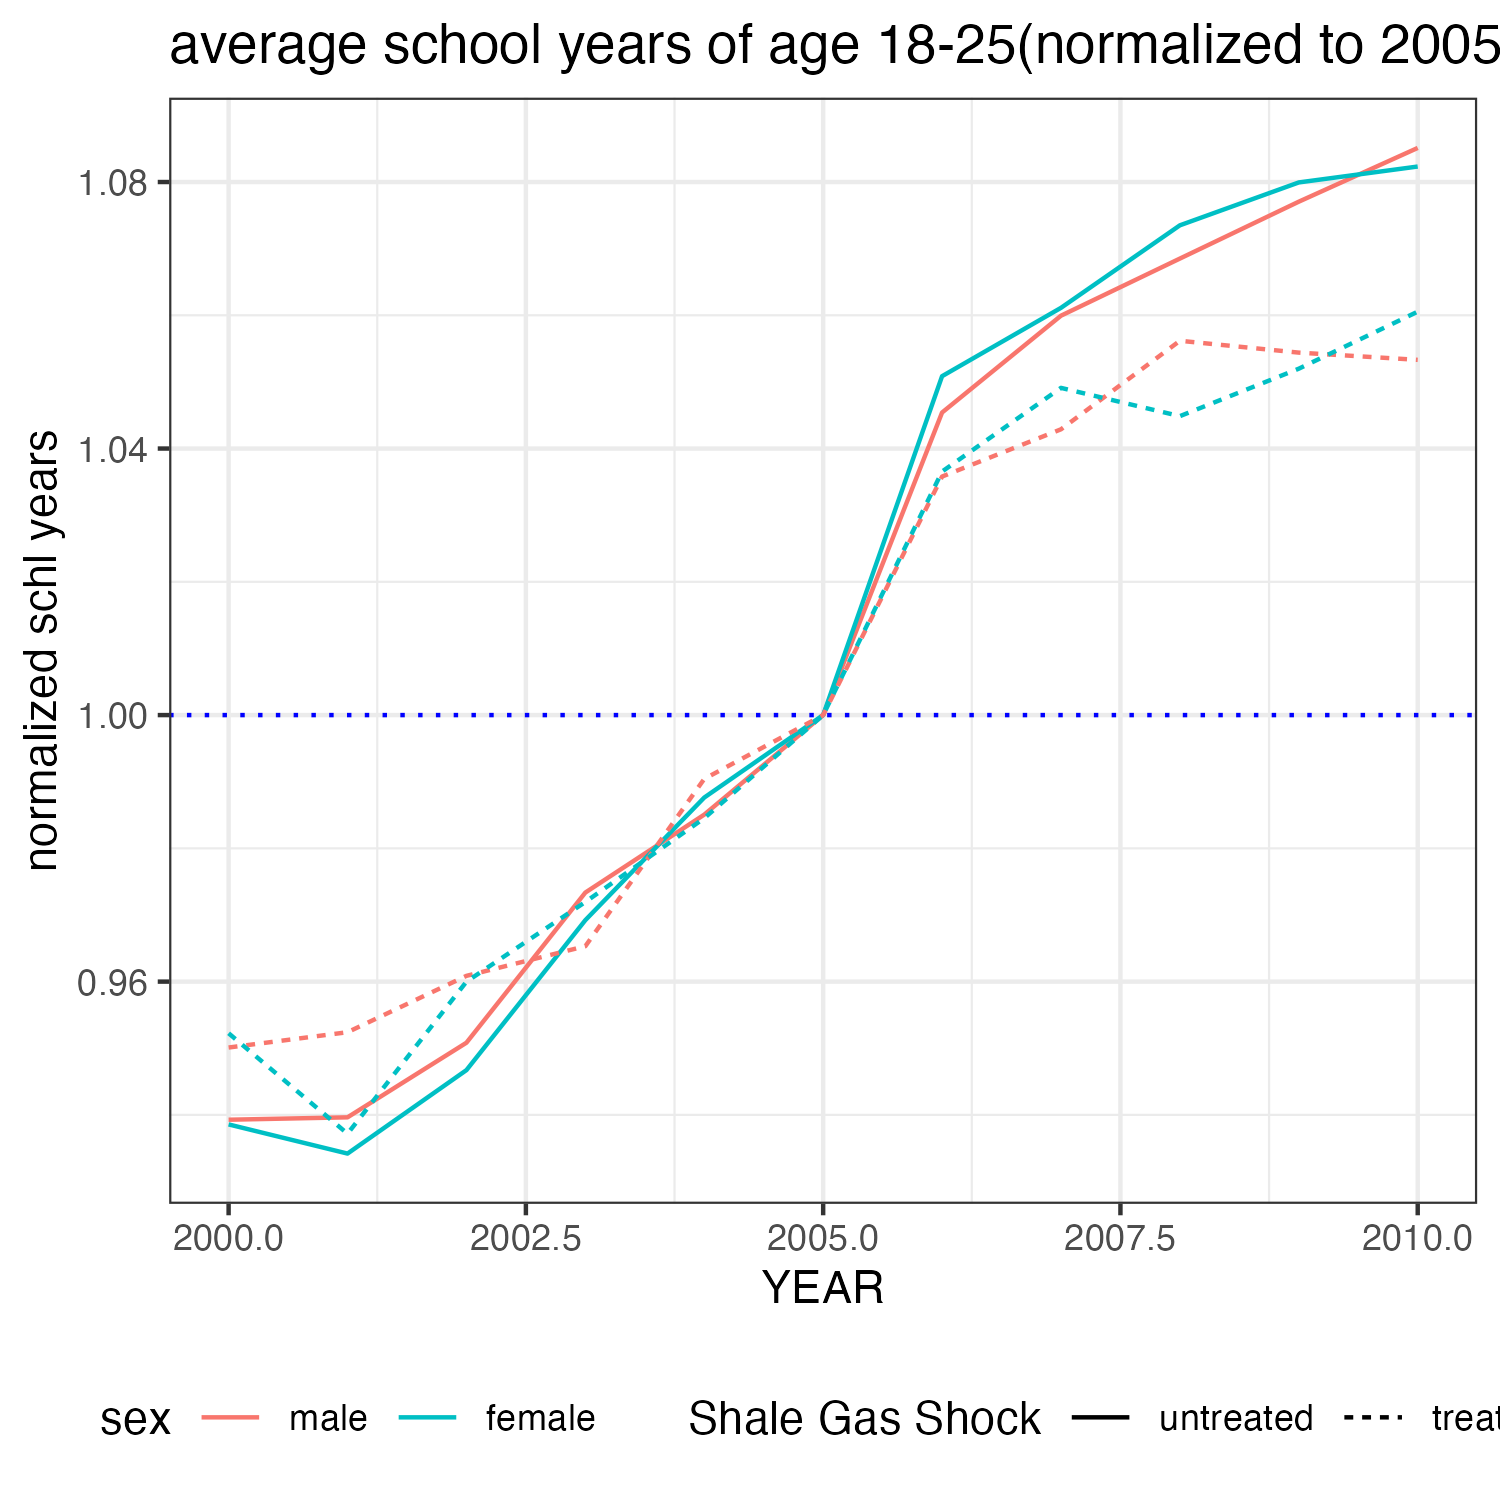
\includegraphics[width=0.4\textwidth]{figures/did-base/fig1.png}
%     \caption{Impact of Shale Gas Boom on Average Schooling Years}
%     \label{fig:did-base-fig1}
%     \begin{minipage}{10cm}
%     \scriptsize
%     Notes:
%     \end{minipage}
% \end{figure}

\begin{figure}[htbp]
    \centering
    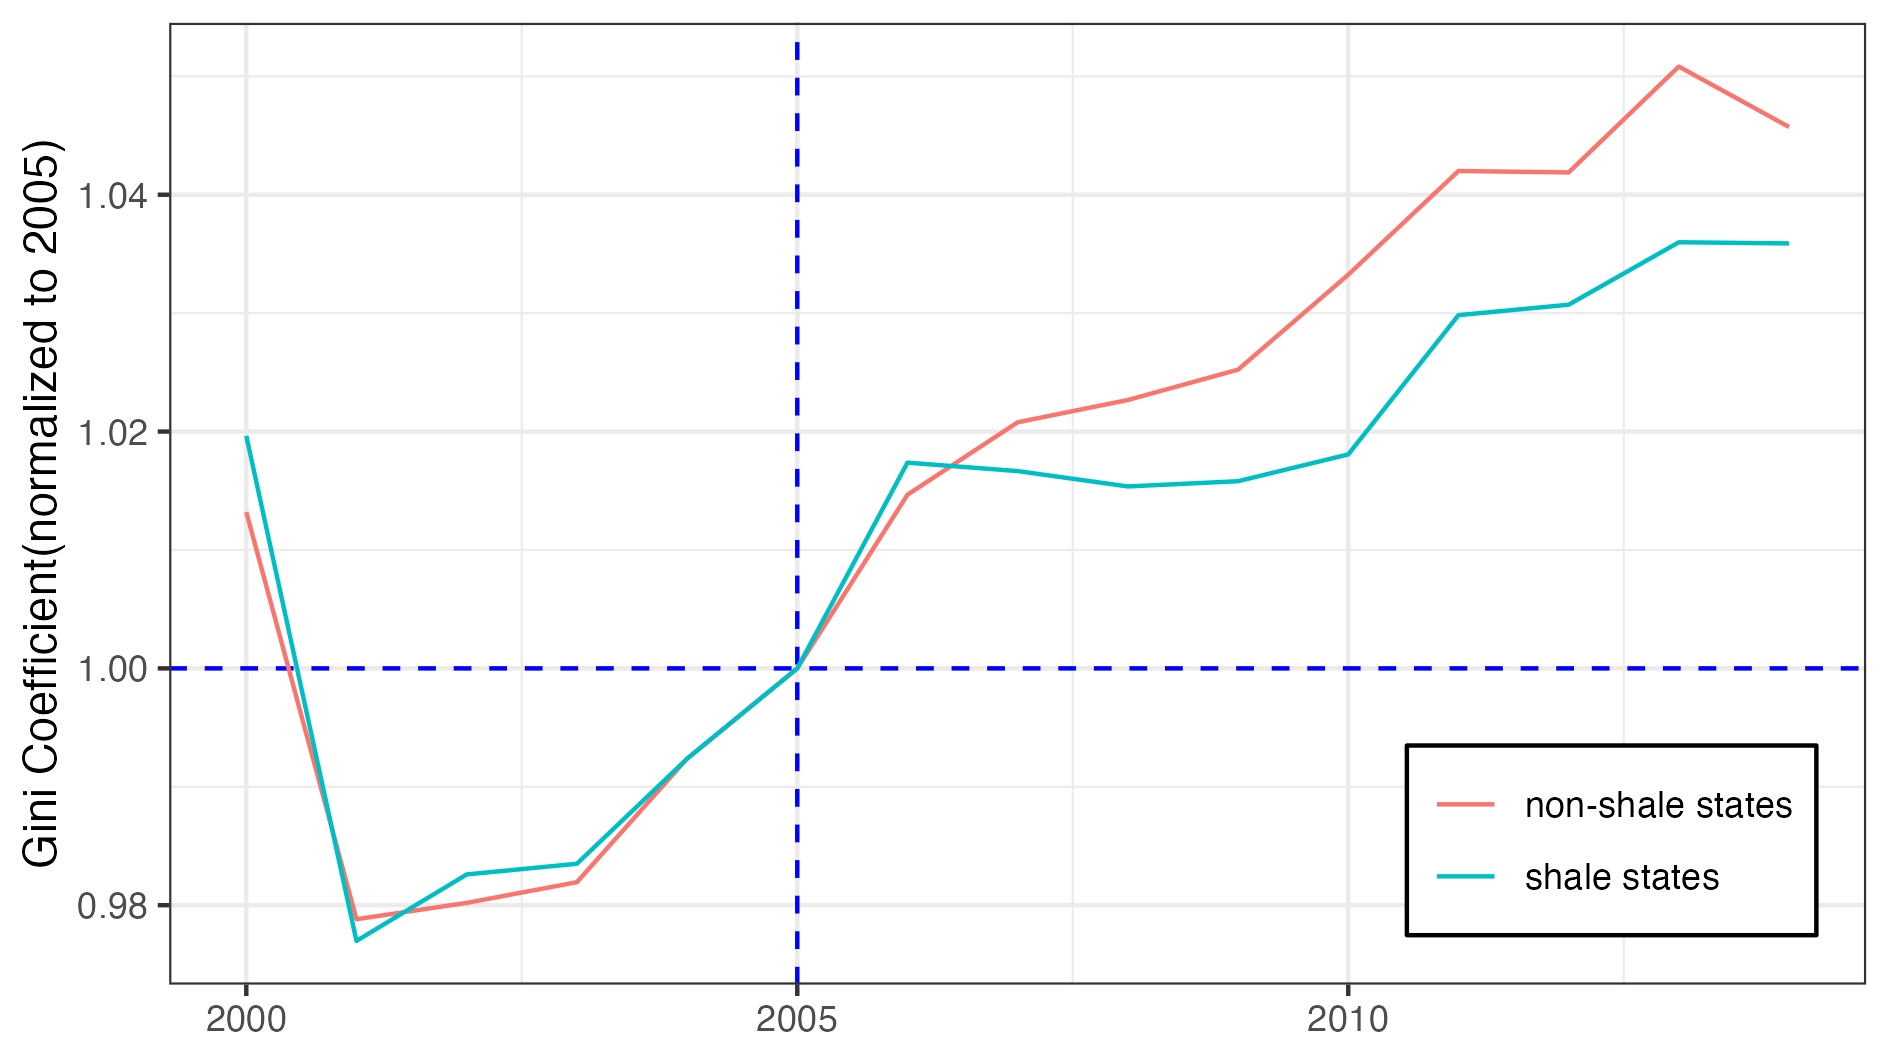
\includegraphics[width=0.7\textwidth]{figures/gini.png}
    \captionsetup{width=0.7\textwidth}
    \caption{Gini Coefficient by Treatment Status}
    \label{fig:gini}
    \begin{minipage}{0.7\textwidth}
    \scriptsize
    Notes: The Gini coefficient is computed within the ACS yearly data for each state, based on individual yearly income. 
    Individuals without income infomrmation or with negative net income are excluded from the calculation, and the Gini coefficient in the figure 
    is normalized to the 2005 level of each respective group.
    \end{minipage}
\end{figure}

\begin{figure}[htbp]
    \centering
    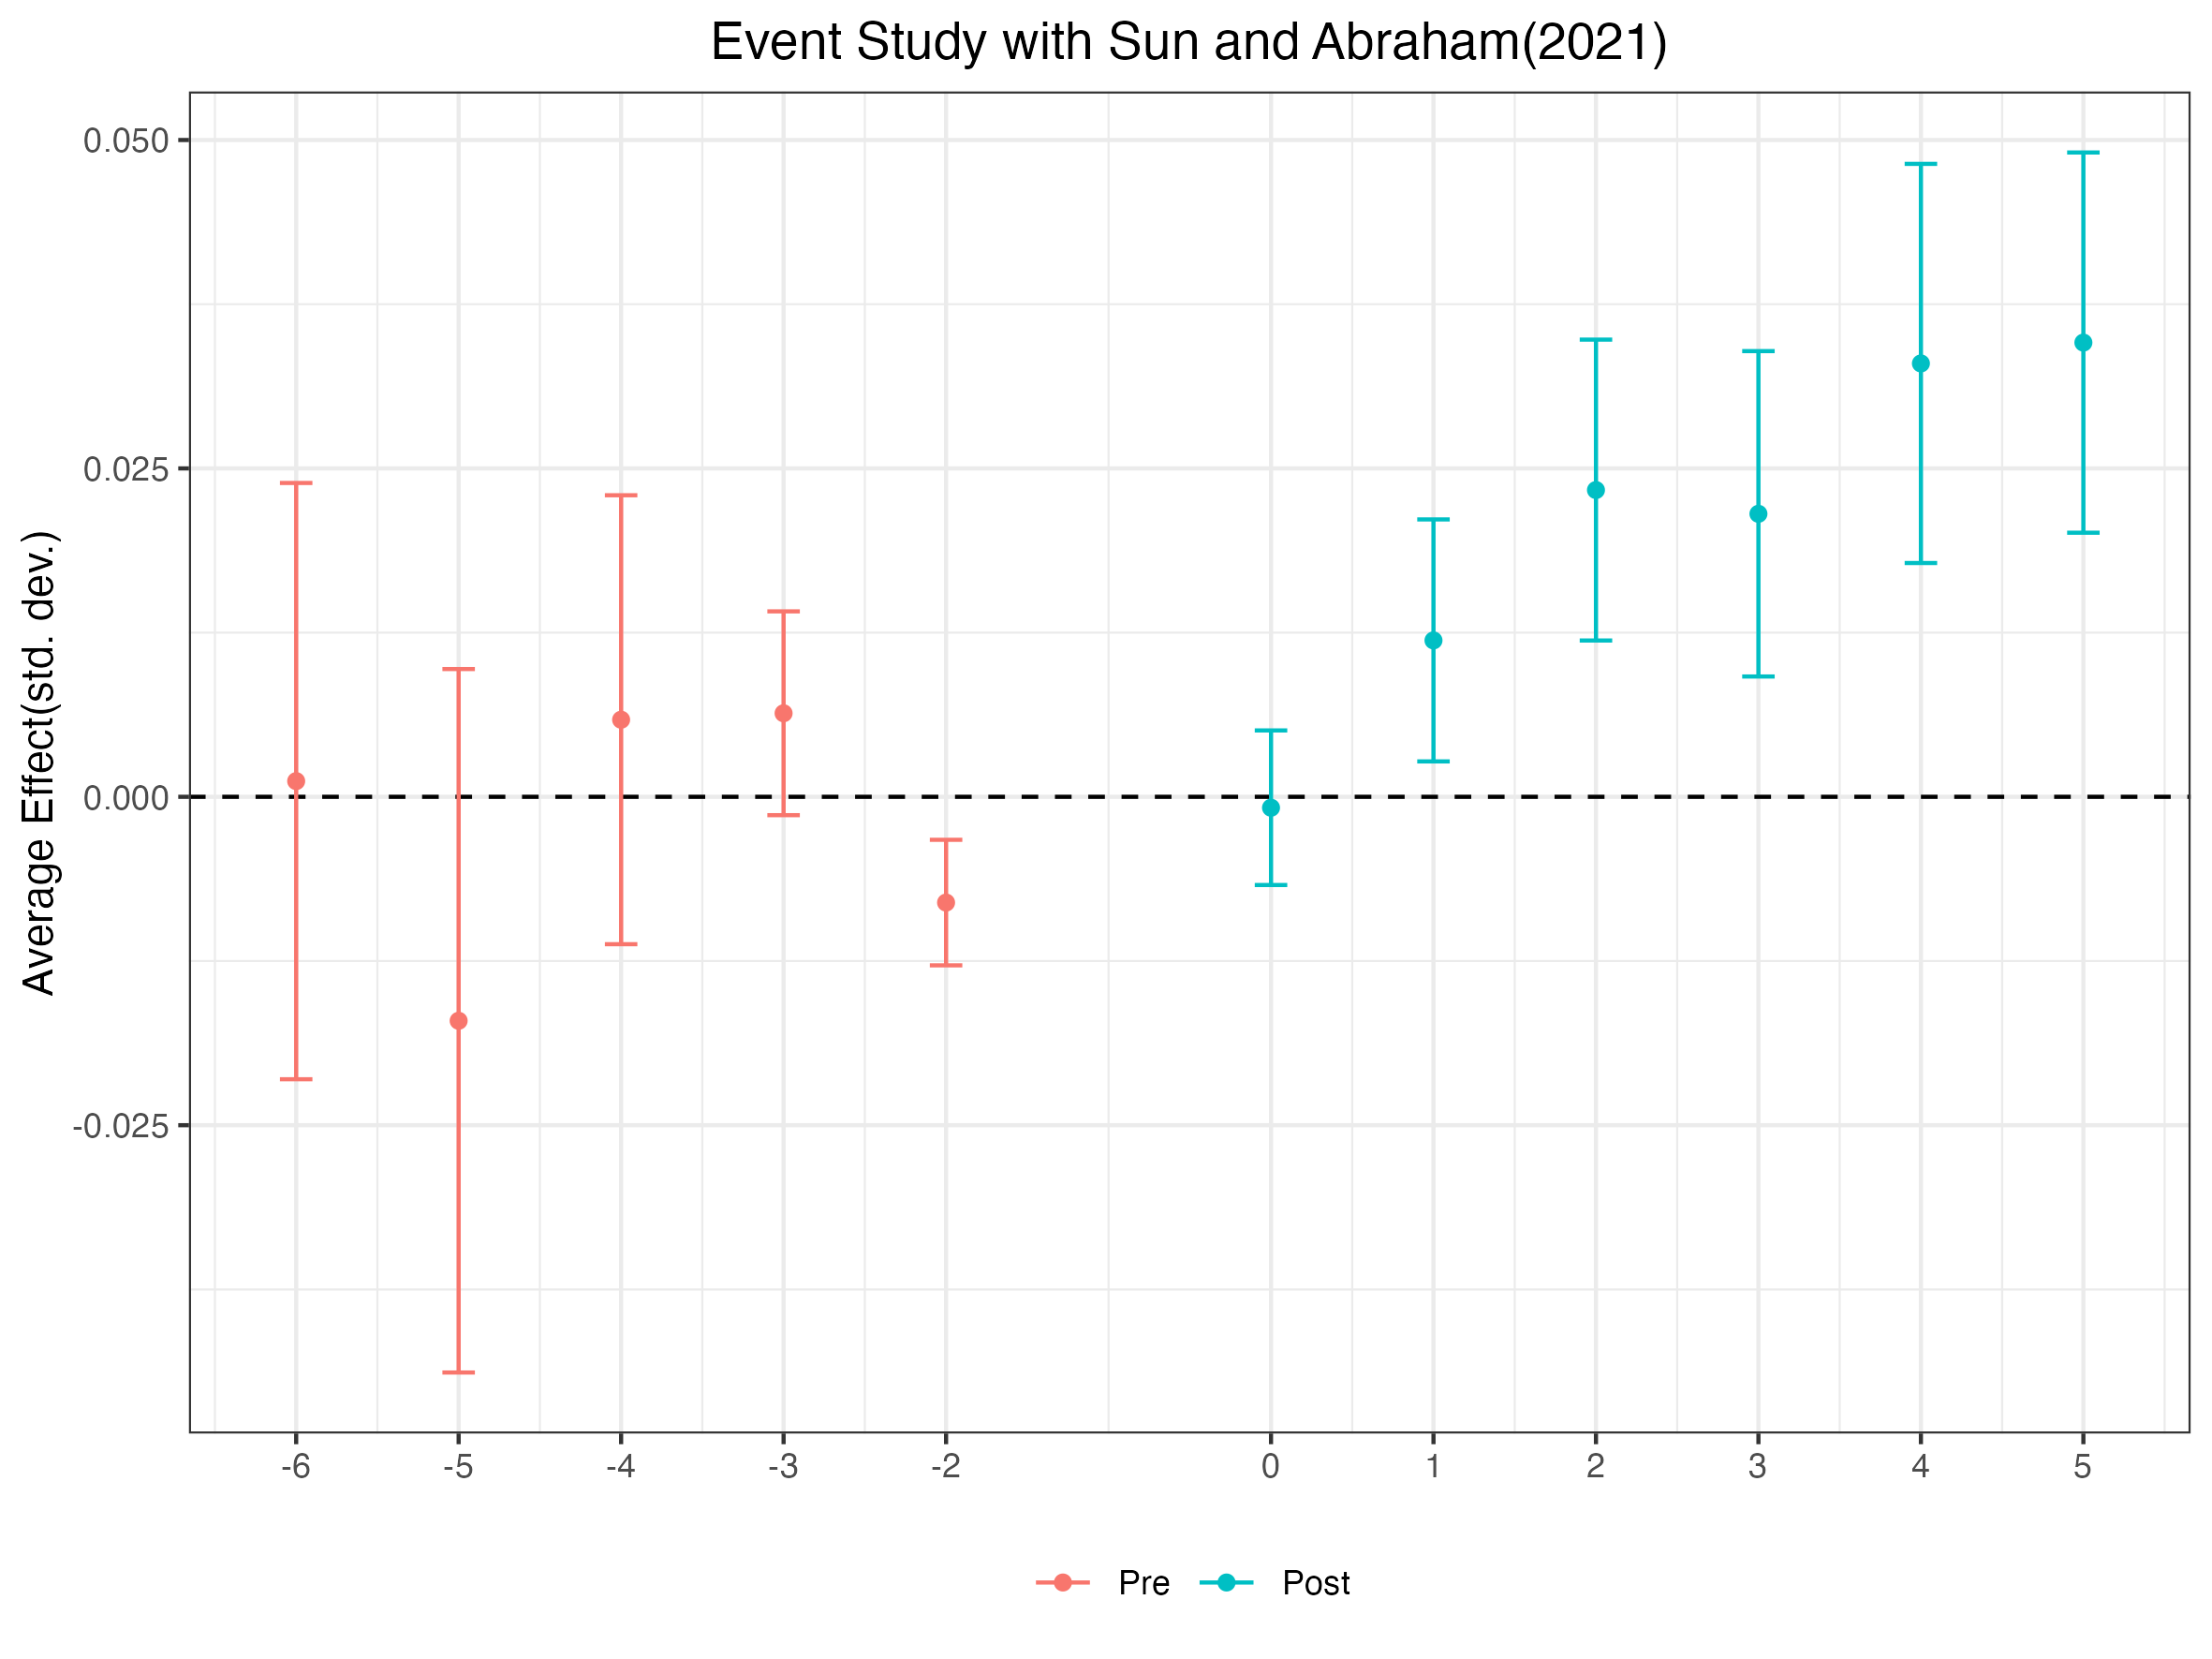
\includegraphics[width=0.7\textwidth, height=8.5cm]{figures/did-base/sadid(logFTOTINC).png}
    \captionsetup{width=0.7\textwidth}
    \caption{Event Study: Overall Household Income}
    \label{fig:Overall Income}
    \begin{minipage}{0.7\textwidth}
    \scriptsize
    Notes: The figure shows the event study results of the household income based on SA-DiD. 
    The base period is set to the year before the shale boom started in each state.
    The point estimates can be interpreted as the percentage change in household income with respect to the treatment (i.e., the shale boom).
    Standard errors are clustered at the state level and the confidence intervals shown are 95\% confidence intervals.
    \end{minipage}
\end{figure}

\begin{figure}[htbp]
    \centering
    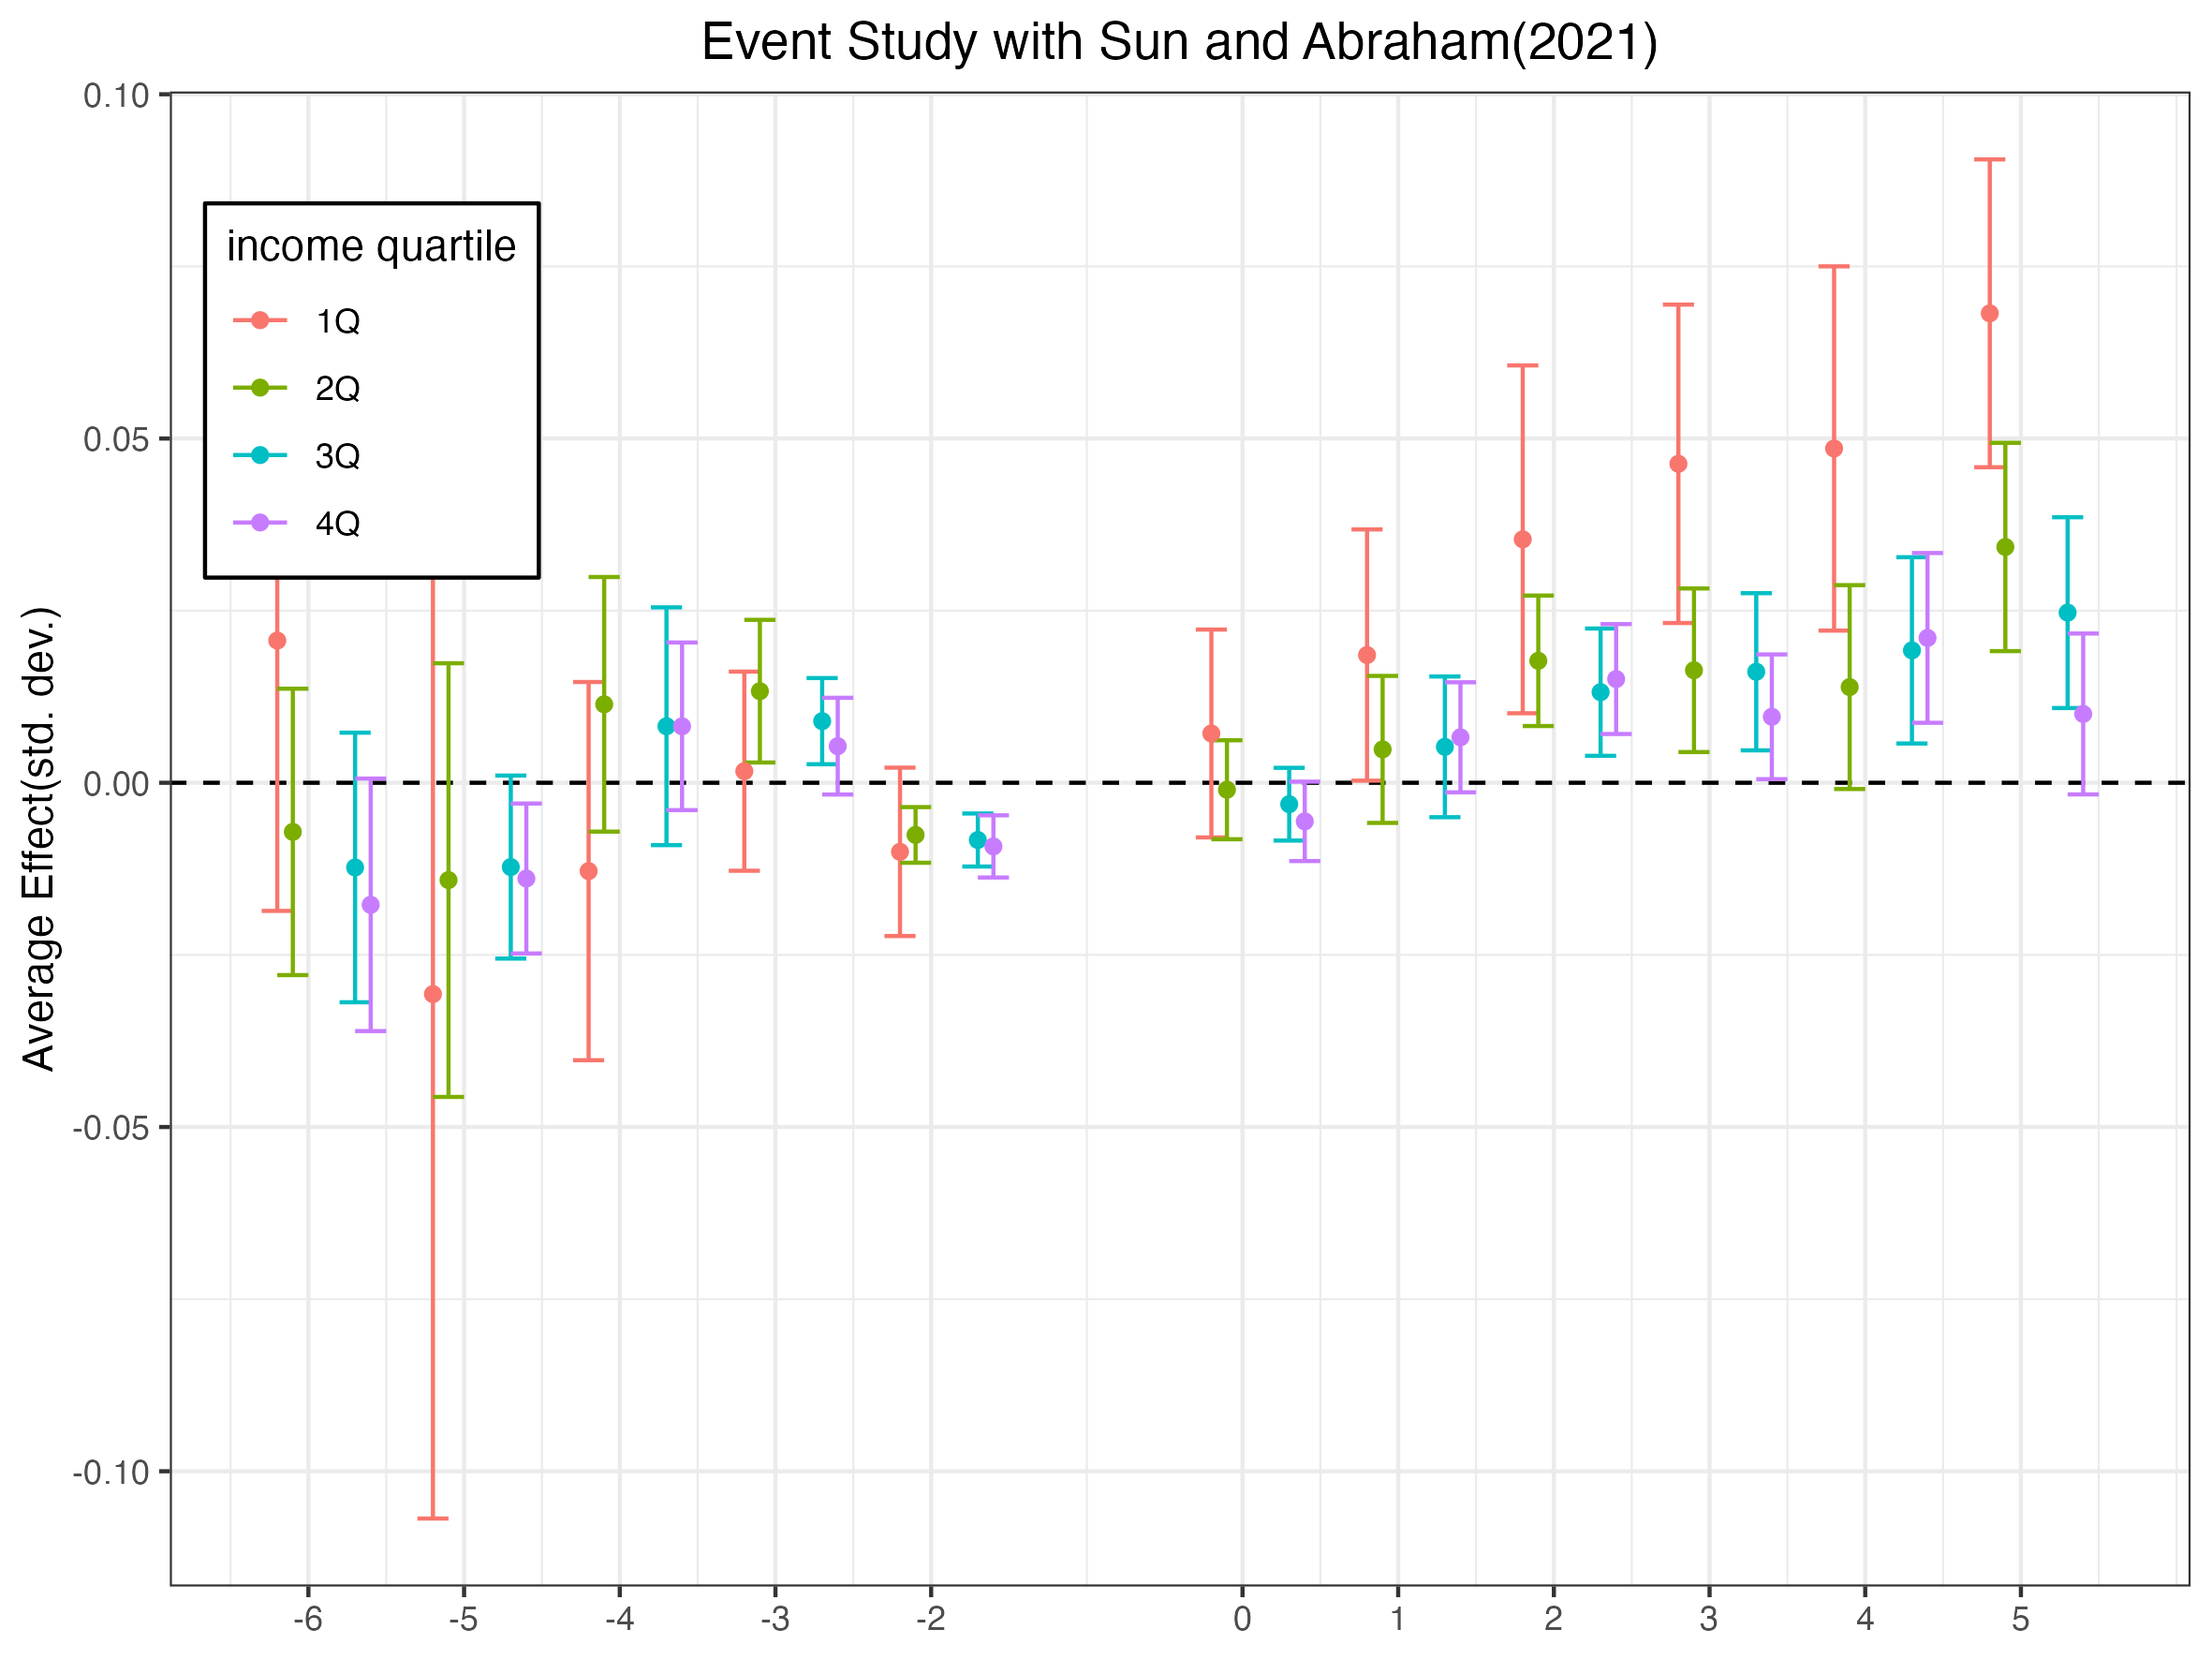
\includegraphics[width=0.7\textwidth]{figures/did-base/sadid(logFTOTINC - by income quartile).png}
    \captionsetup{width=0.7\textwidth}
    \caption{Event Study: Household Income by Quartile}
    \label{fig:Income by Quartile}
    \begin{minipage}{0.7\textwidth}
    \scriptsize
    Notes: The figure shows the event study results of the household income by income quartile based on SA-DiD. 
    The base period is set to the year before the shale boom started in each state.
    The point estimates can be interpreted as the percentage change in household income with respect to the treatment (i.e., the shale boom).
    Standard errors are clustered at the state level and the confidence intervals shown are 95\% confidence intervals.
    Also, note that the cutoffs for income quartiles are nation-level quartiles adjusted by the sampling weights and is fluctuant across years.
    \end{minipage}
\end{figure}

\begin{figure}[htbp]
    \centering
    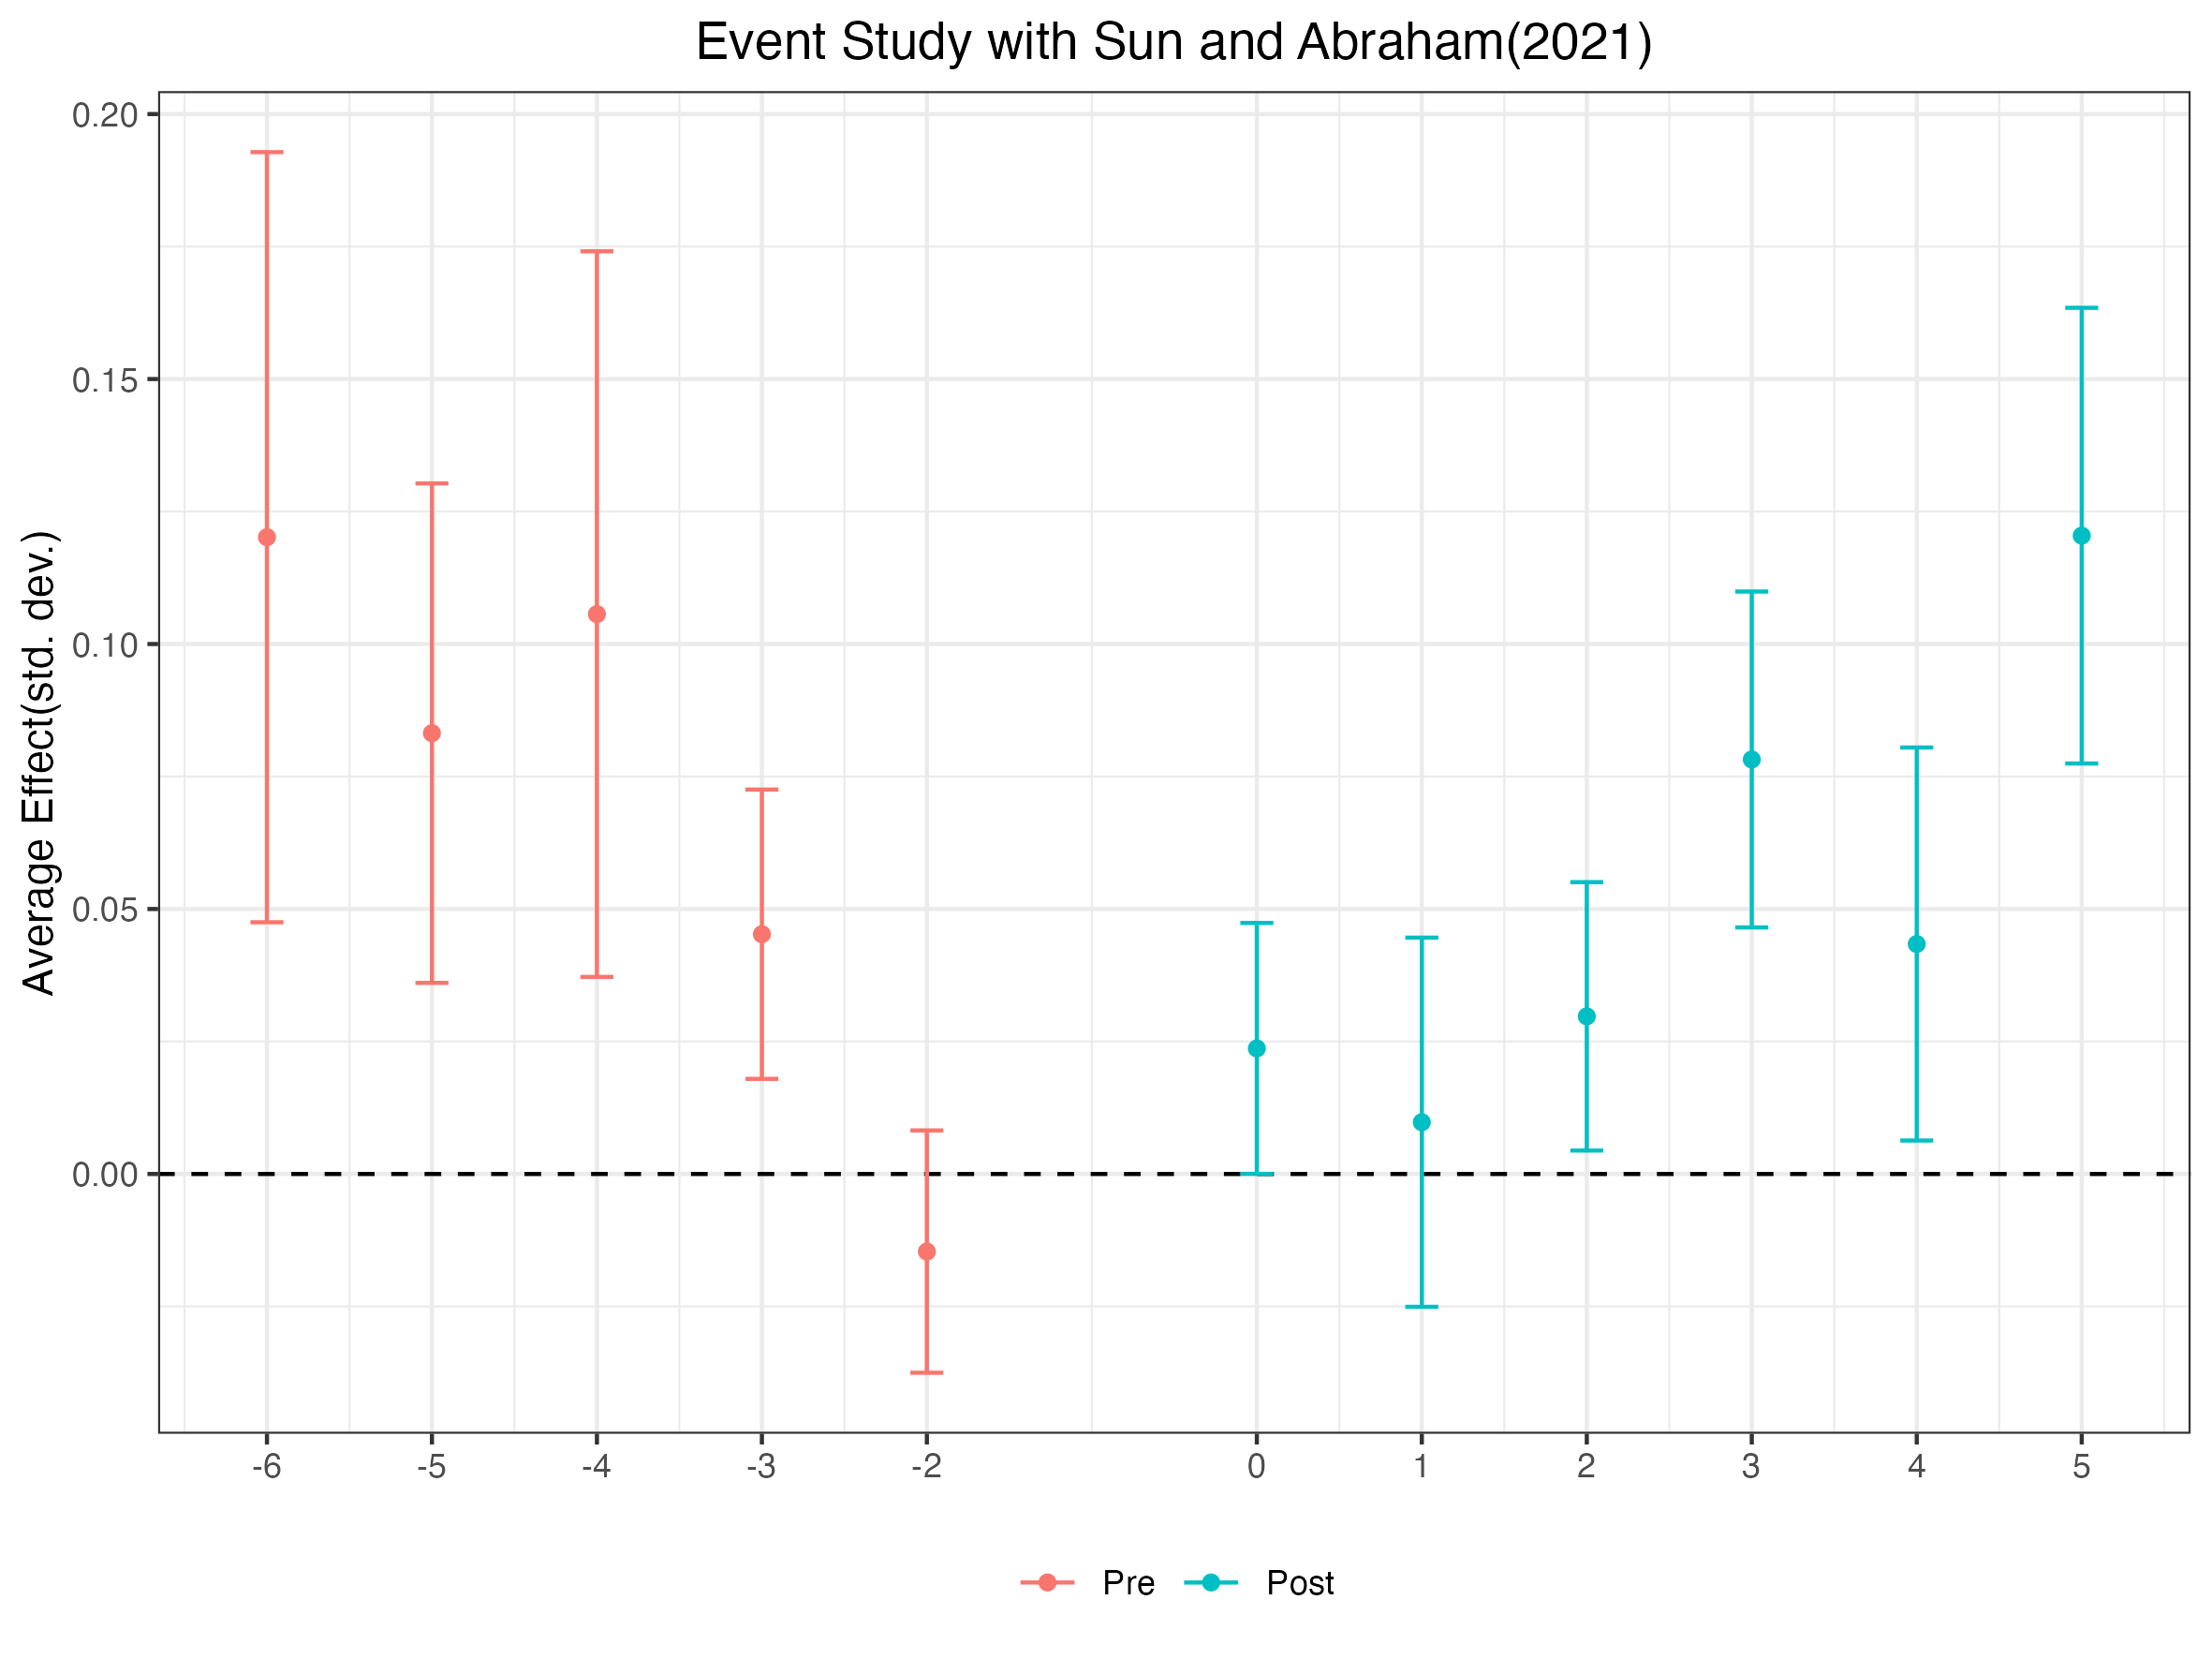
\includegraphics[width=0.7\textwidth, height=8.5cm]{figures/did-base/sadid(college enrollment).png}
    \captionsetup{width=0.7\textwidth}
    \caption{Event Study: Overall College Enrollment}
    \label{fig:college shares}
    \begin{minipage}{0.7\textwidth}
    \scriptsize
    Notes: The figure shows the event study results of the college enrollment among individuals between age 18 and 24 (inclusive) based on SA-DiD. 
    The base period is set to the year before the shale boom started in each state.
    The point estimates can be interpreted as the percentage point change in college enrollment status with respect to the treatment (i.e., the shale boom).
    Standard errors are clustered at the state level and the confidence intervals shown are 95\% confidence intervals.
    \end{minipage}
\end{figure}

\begin{figure}[htbp]
    \centering
    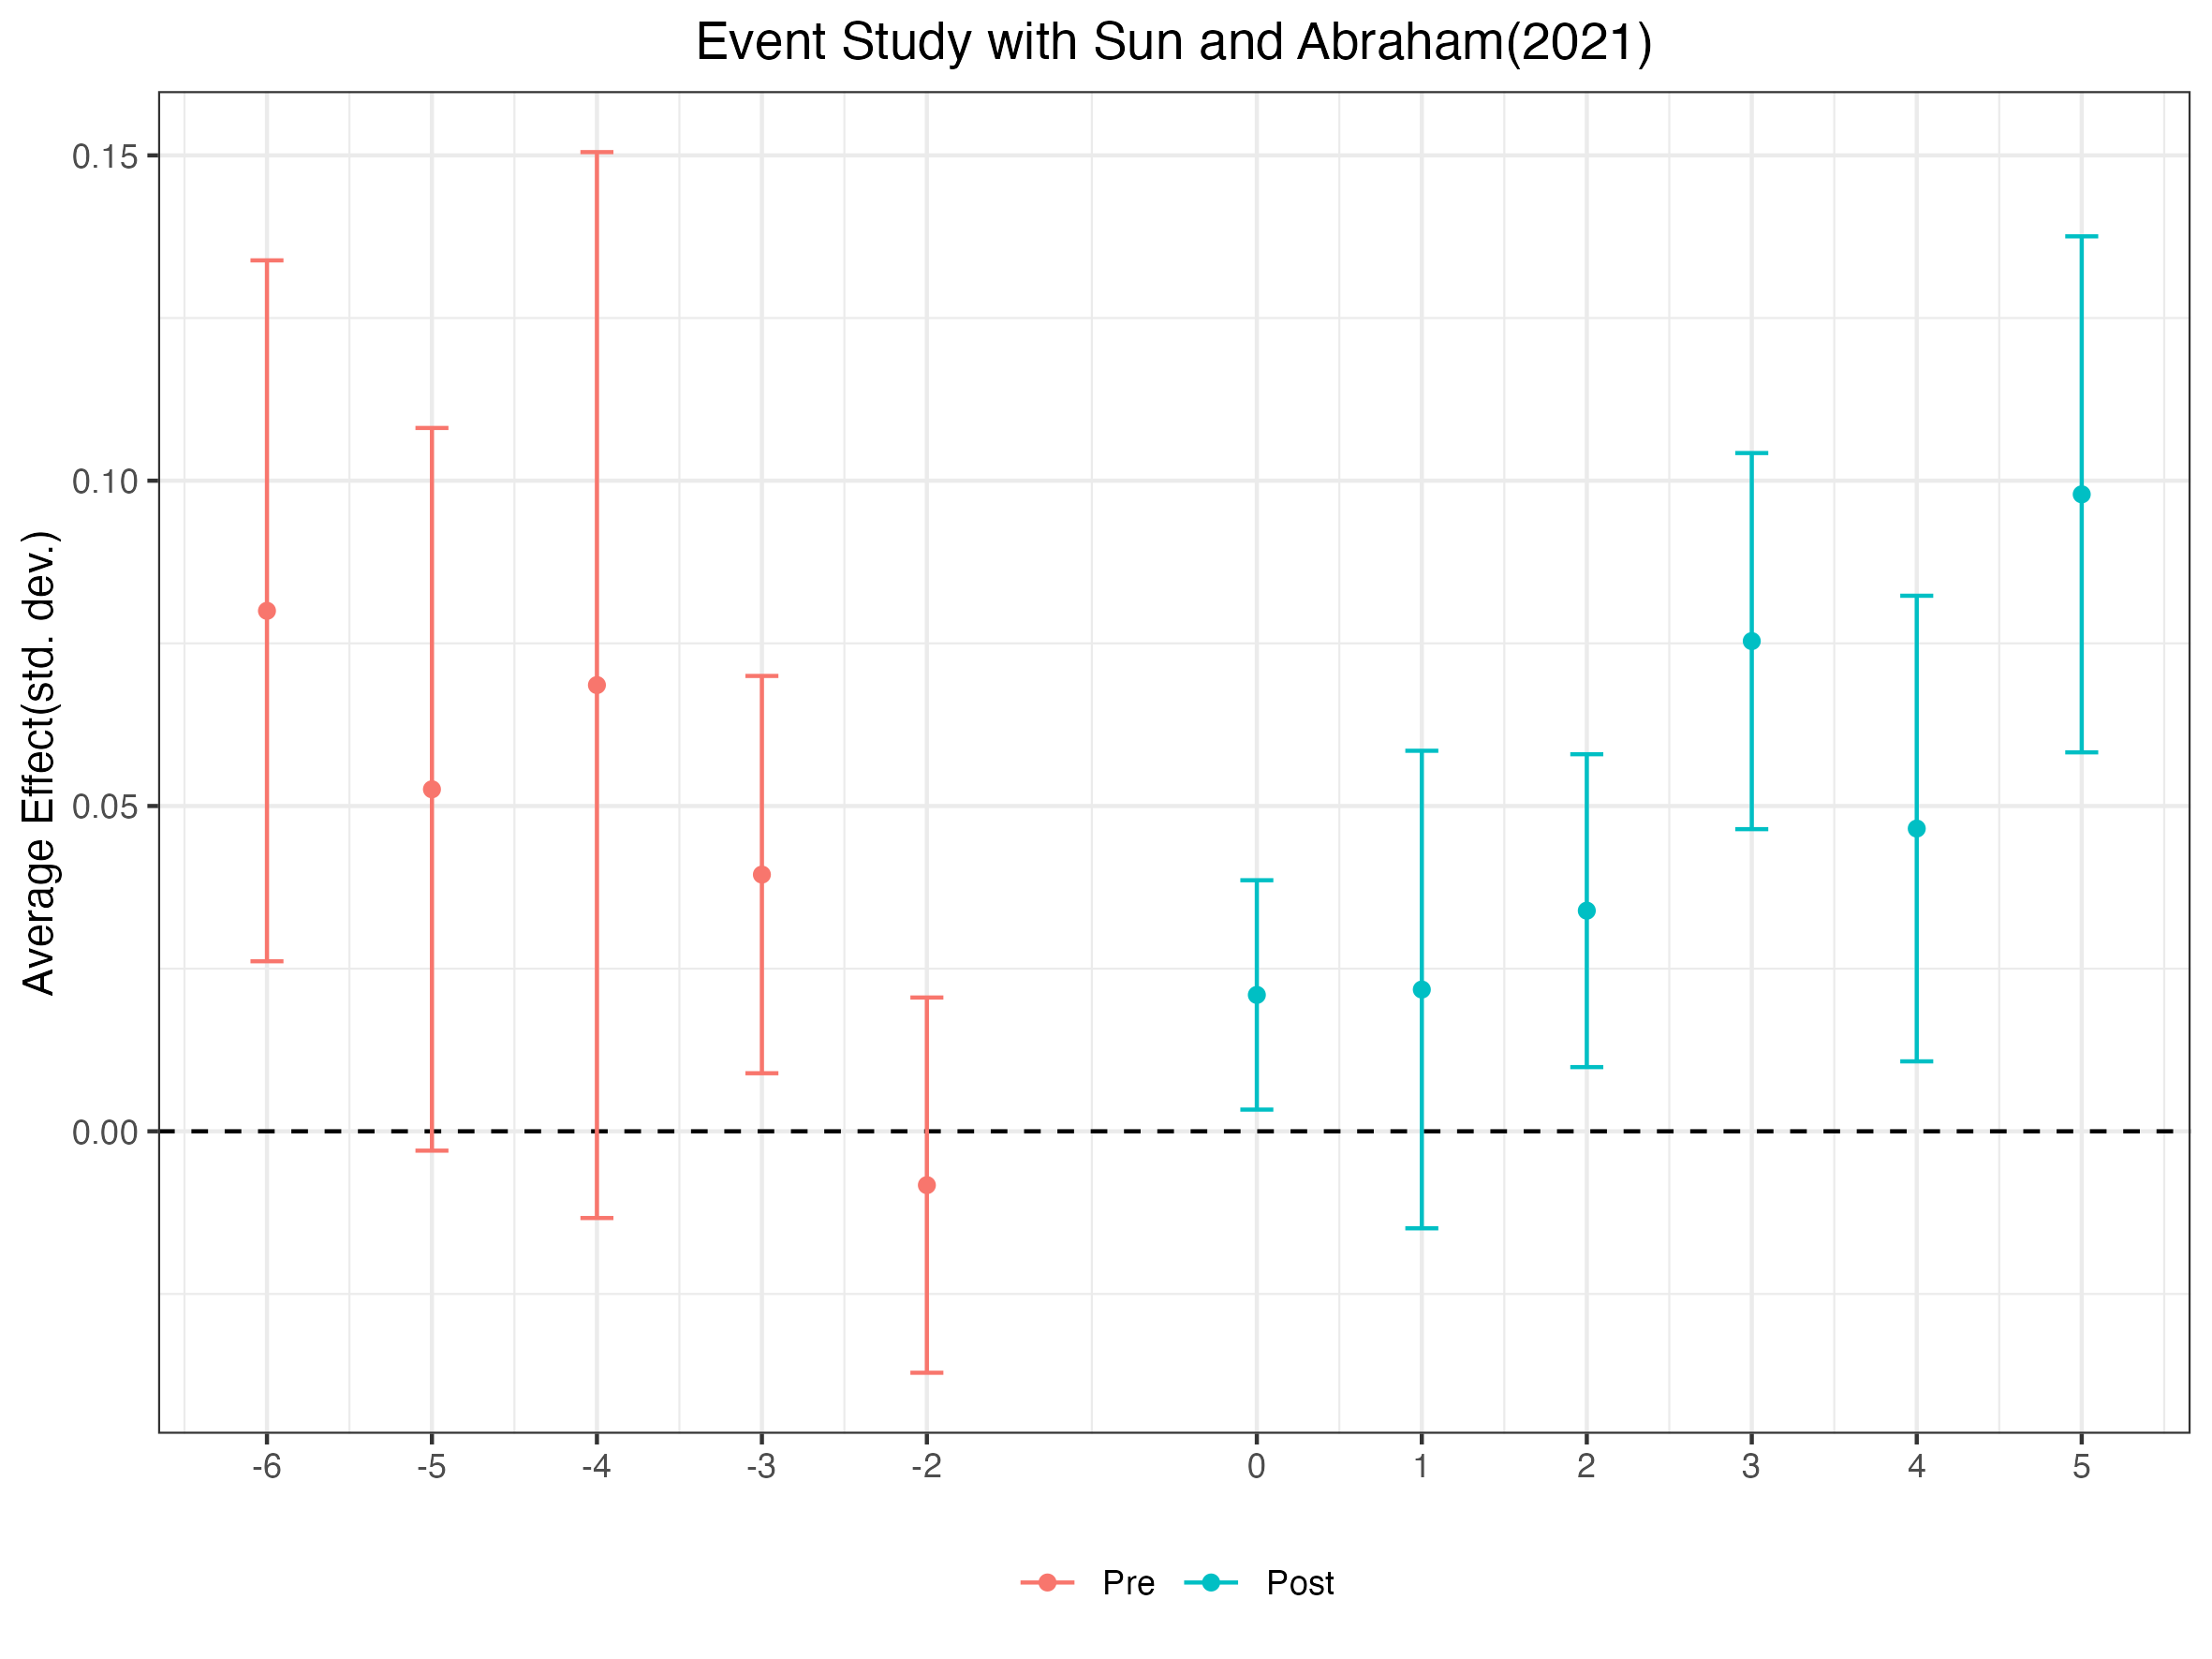
\includegraphics[width=0.7\textwidth, height=8.5cm]{figures/did-base/sadid(college enrollment - controls).png}
    \captionsetup{width=0.7\textwidth}
    \caption{Event Study: Overall College Enrollment (with Controls)}
    \label{fig:college shares-controls}
    \begin{minipage}{0.7\textwidth}
    \scriptsize
    Notes: The figure shows the event study results of the college enrollment among individuals between age 18 and 24 (inclusive) based on SA-DiD with covariates. 
    Covariates include sex, race, and household income of the individual.
    The base period is set to the year before the shale boom started in each state.
    The point estimates can be interpreted as the percentage point change in college enrollment status with respect to the treatment (i.e., the shale boom).
    Standard errors are clustered at the state level and the confidence intervals shown are 95\% confidence intervals.
    \end{minipage}
\end{figure}

\begin{figure}[htbp]
    \centering
    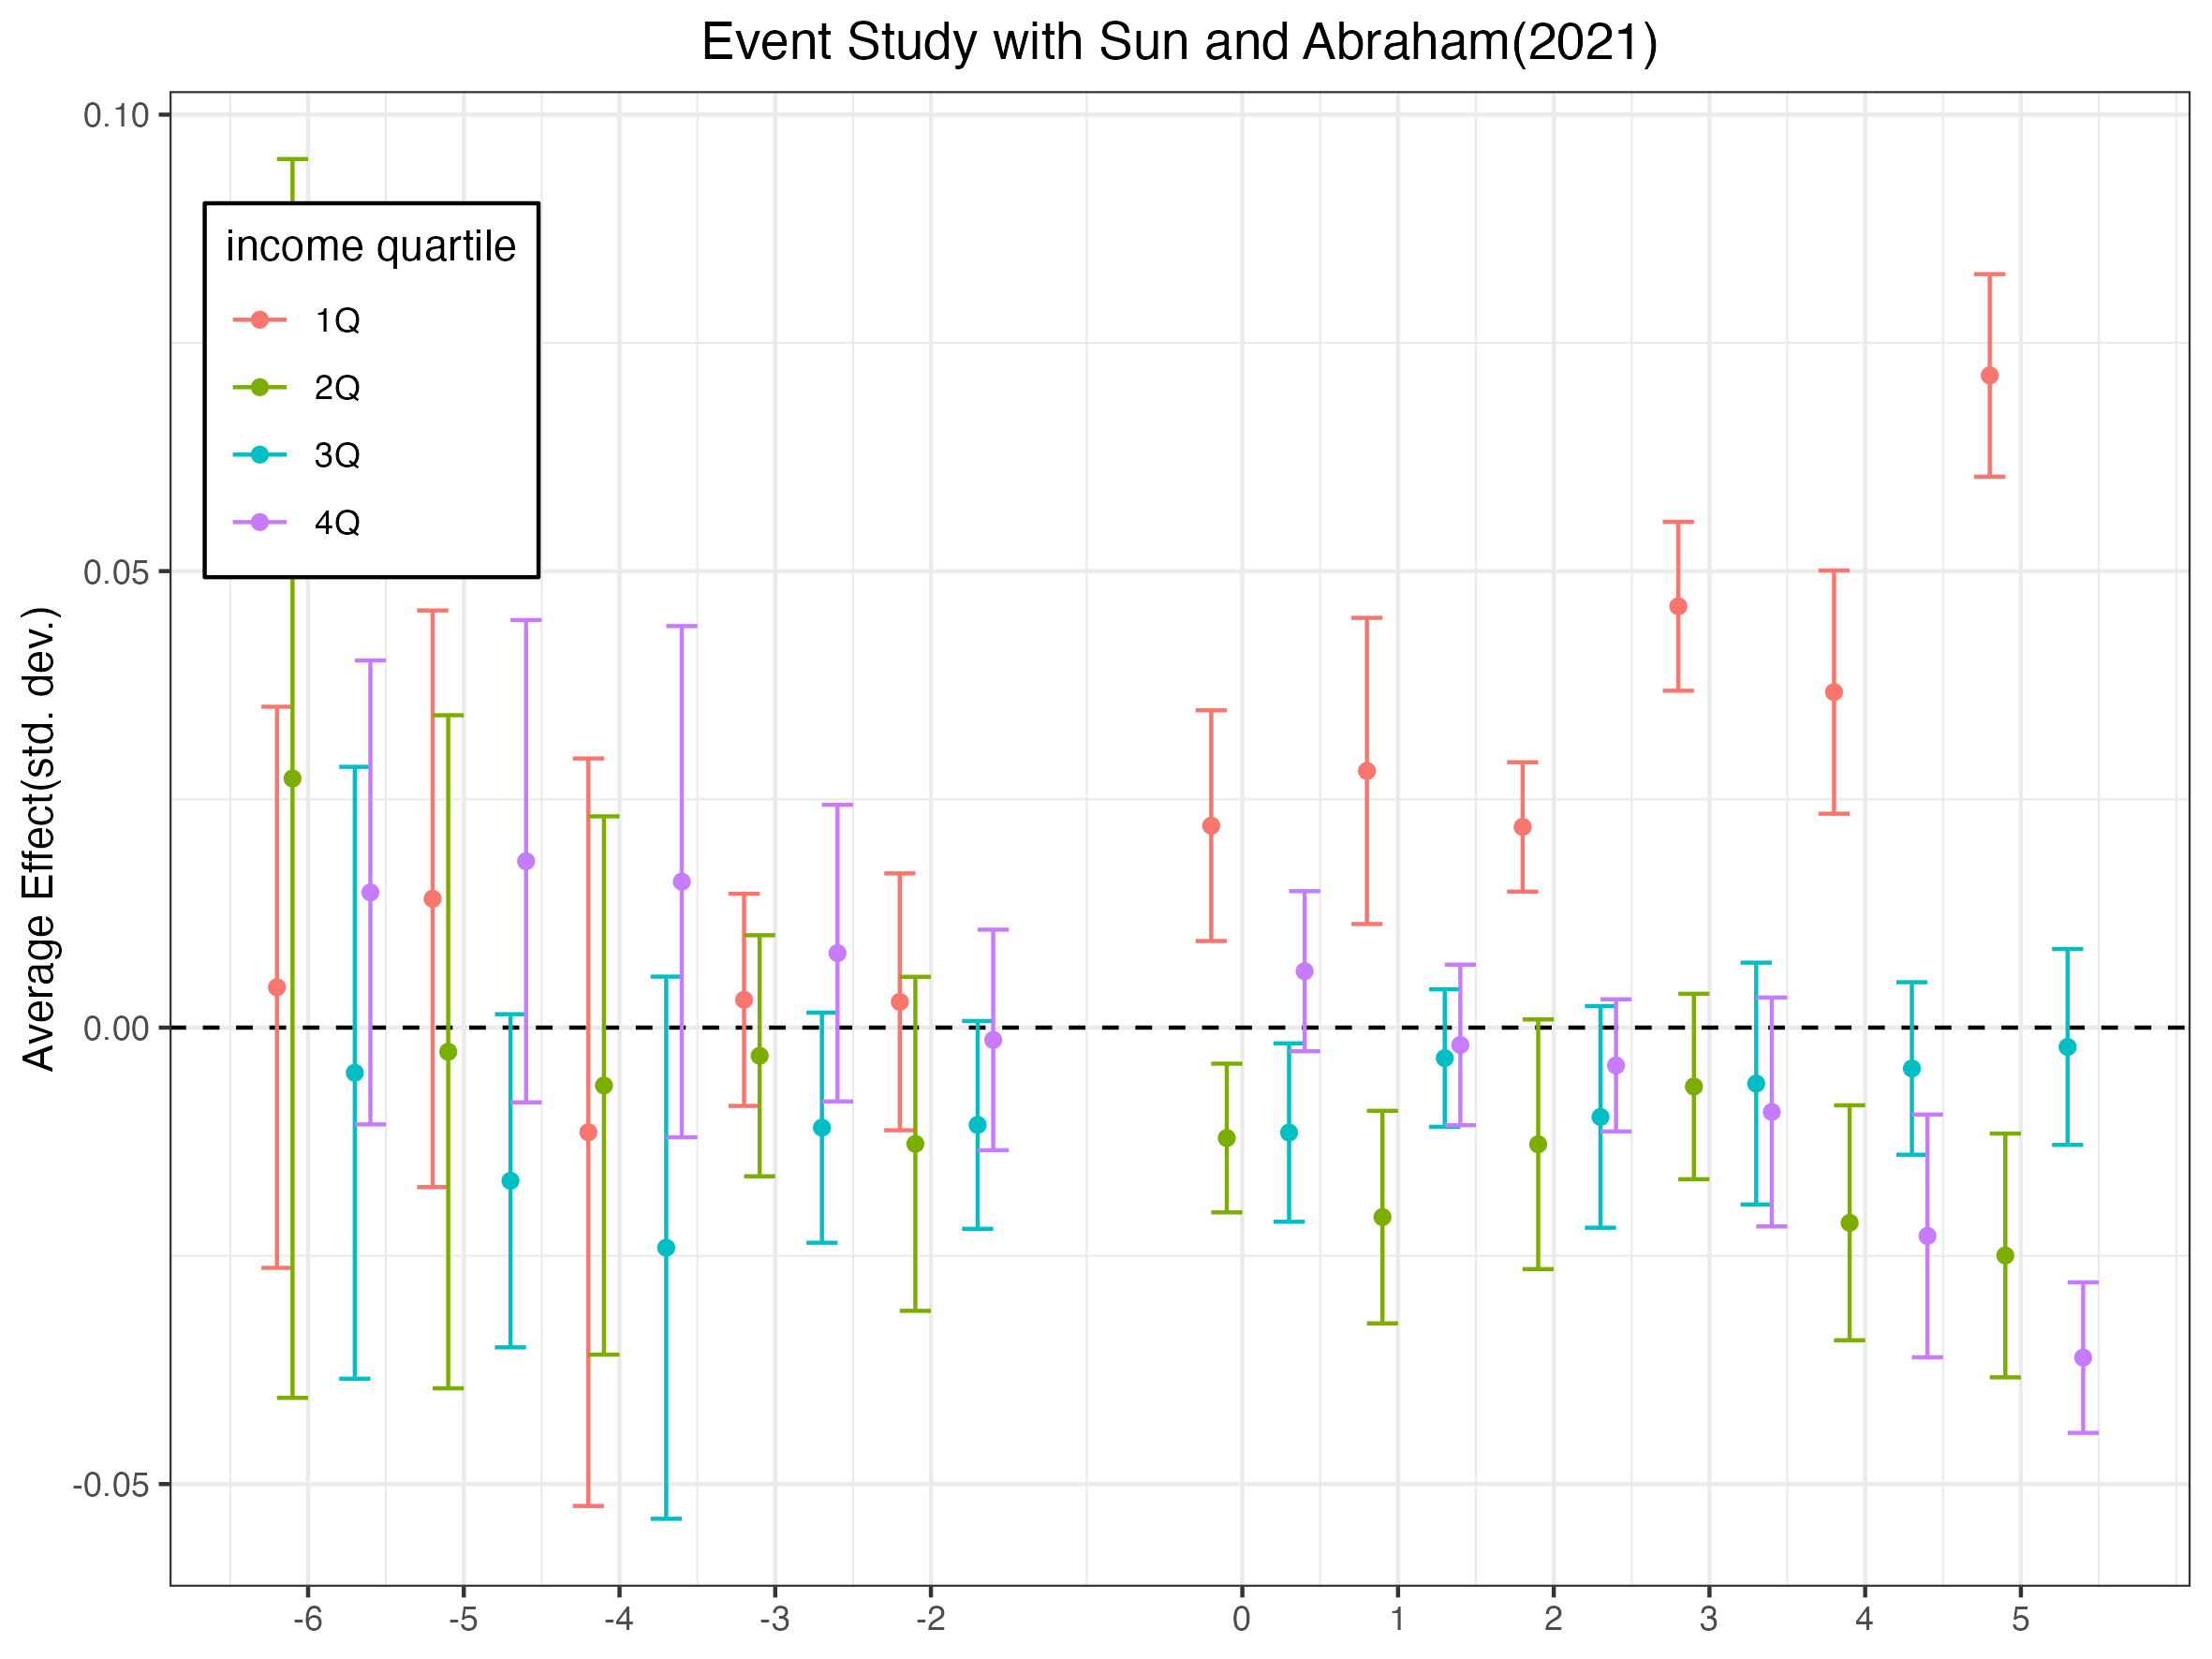
\includegraphics[width=0.7\textwidth]{figures/did-base/sadid(college share - by income quartile).png}
    \captionsetup{width=0.7\textwidth}
    \caption{Event Study: College Enrollment by Household Income Quartile}
    \label{fig:college enrollment}
    \begin{minipage}{0.7\textwidth}
    \scriptsize
    Notes: The figure shows the event study results of the college enrollment among individuals between age 18 and 24 (inclusive) by family income quartile based on SA-DiD. 
    The base period is set to the year before the shale boom started in each state.
    The point estimates can be interpreted as the percentage point change in college enrollment status with respect to the treatment (i.e., the shale boom).
    Standard errors are clustered at the state level and the confidence intervals shown are 95\% confidence intervals.
    Also, note that the cutoffs for income quartiles are nation-level quartiles adjusted by the sampling weights and is fluctuant across years.
    \end{minipage}
\end{figure}

\begin{figure}[htbp]
    \centering
    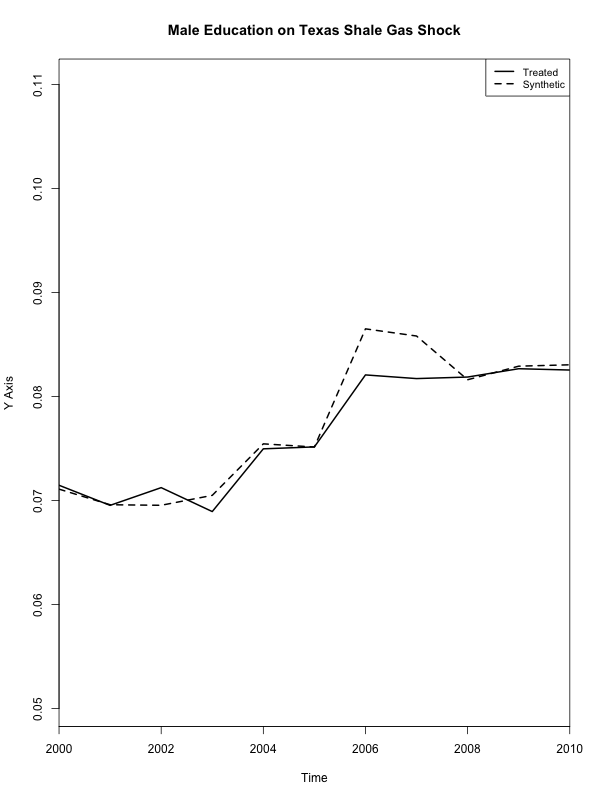
\includegraphics[width=0.7\textwidth]{figures/scm/fig3_v4.png}
    \captionsetup{width=0.7\textwidth}
    \caption{SCM Male Education}
    \label{fig:SCM male}
    \begin{minipage}{0.7\textwidth}
    \scriptsize
    Notes: The figure shows the synthetic control estimates of the college enrollment shares among
    males between age 18 and 24 (inclusive) in Texas, where the solid line represents Texas (the treated unit), and the dashed line corresponds to the synthetic control group.
    The weights for the synthetic control group are based on race composition, minor ratio (i.e., the ratio of individuals aged 0-17 to the total population), and population size
    in the pre-treatment period, which is defined as 2000 to 2005,
    inclusively.
    \end{minipage}
\end{figure}

\begin{figure}[htbp]
    \centering
    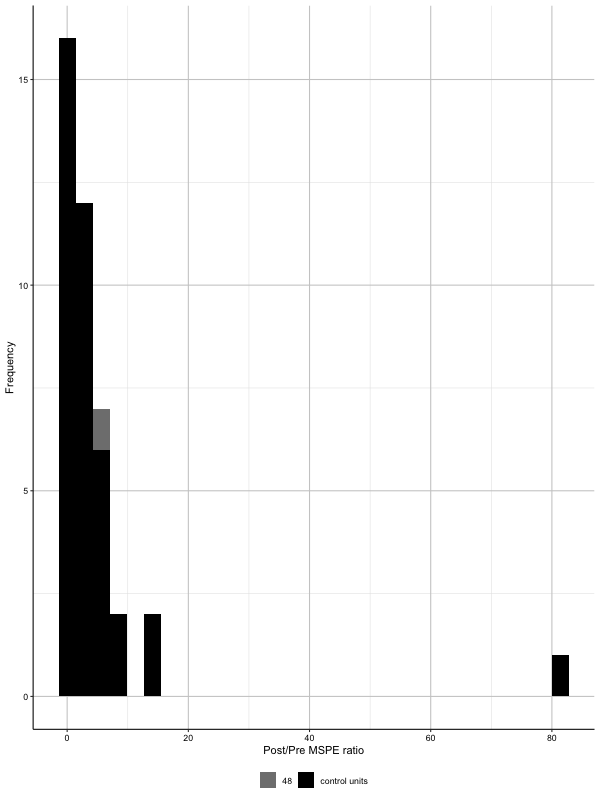
\includegraphics[width=0.7\textwidth]{figures/scm/fig3-mspe_v4.png}
    \captionsetup{width=0.7\textwidth}
    \caption{SCM Male Education MSPE}
    \label{fig:SCM male MSPE}
    \begin{minipage}{0.7\textwidth}
    \scriptsize
    Notes: The figure shows the post-treatment to pre-treatment mean squared prediction error (MSPE) ratio.
    The x-axis represents the MSPE ratio, and the y-axis represents the  frequency of the MSPE ratio.
    In the figure, the grey bar represents the MSPE ratio of Texas, and the black bars are MSPE ratios from having other states as placebo treated units.
    One can readily notice that the MSPE ratio of Texas is located at the left side of the distribution,
    implying that the actual post-treatment outcomes are predicted well by the synthetic control group;
    thus, the difference in college enrollment shares between Texas and its synthetic counterpart is not 
    unusually large relative to the placebo units whose MSPE ratios are shown in the same plot.
    \end{minipage}
\end{figure}

\begin{figure}[htbp]
    \centering
    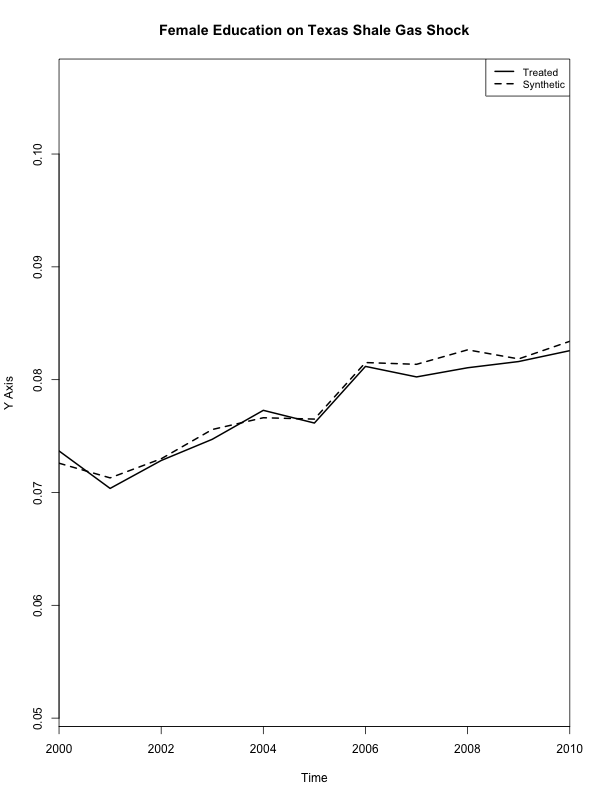
\includegraphics[width=0.7\textwidth]{figures/scm/fig4_v4.png}
    \captionsetup{width=0.7\textwidth}
    \caption{SCM Female Education}
    \label{fig:SCM female}
    \begin{minipage}{0.7\textwidth}
    \scriptsize
    Notes: The figure shows the synthetic control estimates of the college enrollment shares among
    females between age 18 and 24 (inclusive) in Texas, where the solid line represents Texas (the treated unit), and the dashed line corresponds to the synthetic control group.
    The weights for the synthetic control group are based on race composition, minor ratio (i.e., the ratio of individuals aged 0-17 to the total population), and population size
    in the pre-treatment period, which is defined as 2000 to 2005,
    inclusively.
    \end{minipage}
\end{figure}

% \begin{figure}[htbp]
%     \centering
%     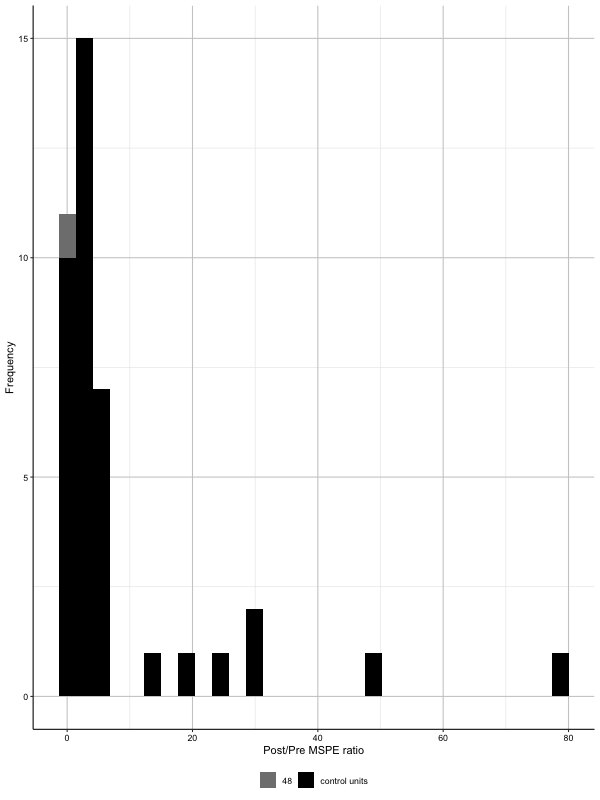
\includegraphics[width=0.7\textwidth]{figures/scm/fig4-mspe_v4.png}
%     \captionsetup{width=0.7\textwidth}
%     \caption{SCM Female Education MSPE}
%     \label{fig:SCM female MSPE}
%     \begin{minipage}{0.7\textwidth}
%     \scriptsize
%     Notes:
%     \end{minipage}
% \end{figure}


\begin{figure}[htbp]
    \centering
    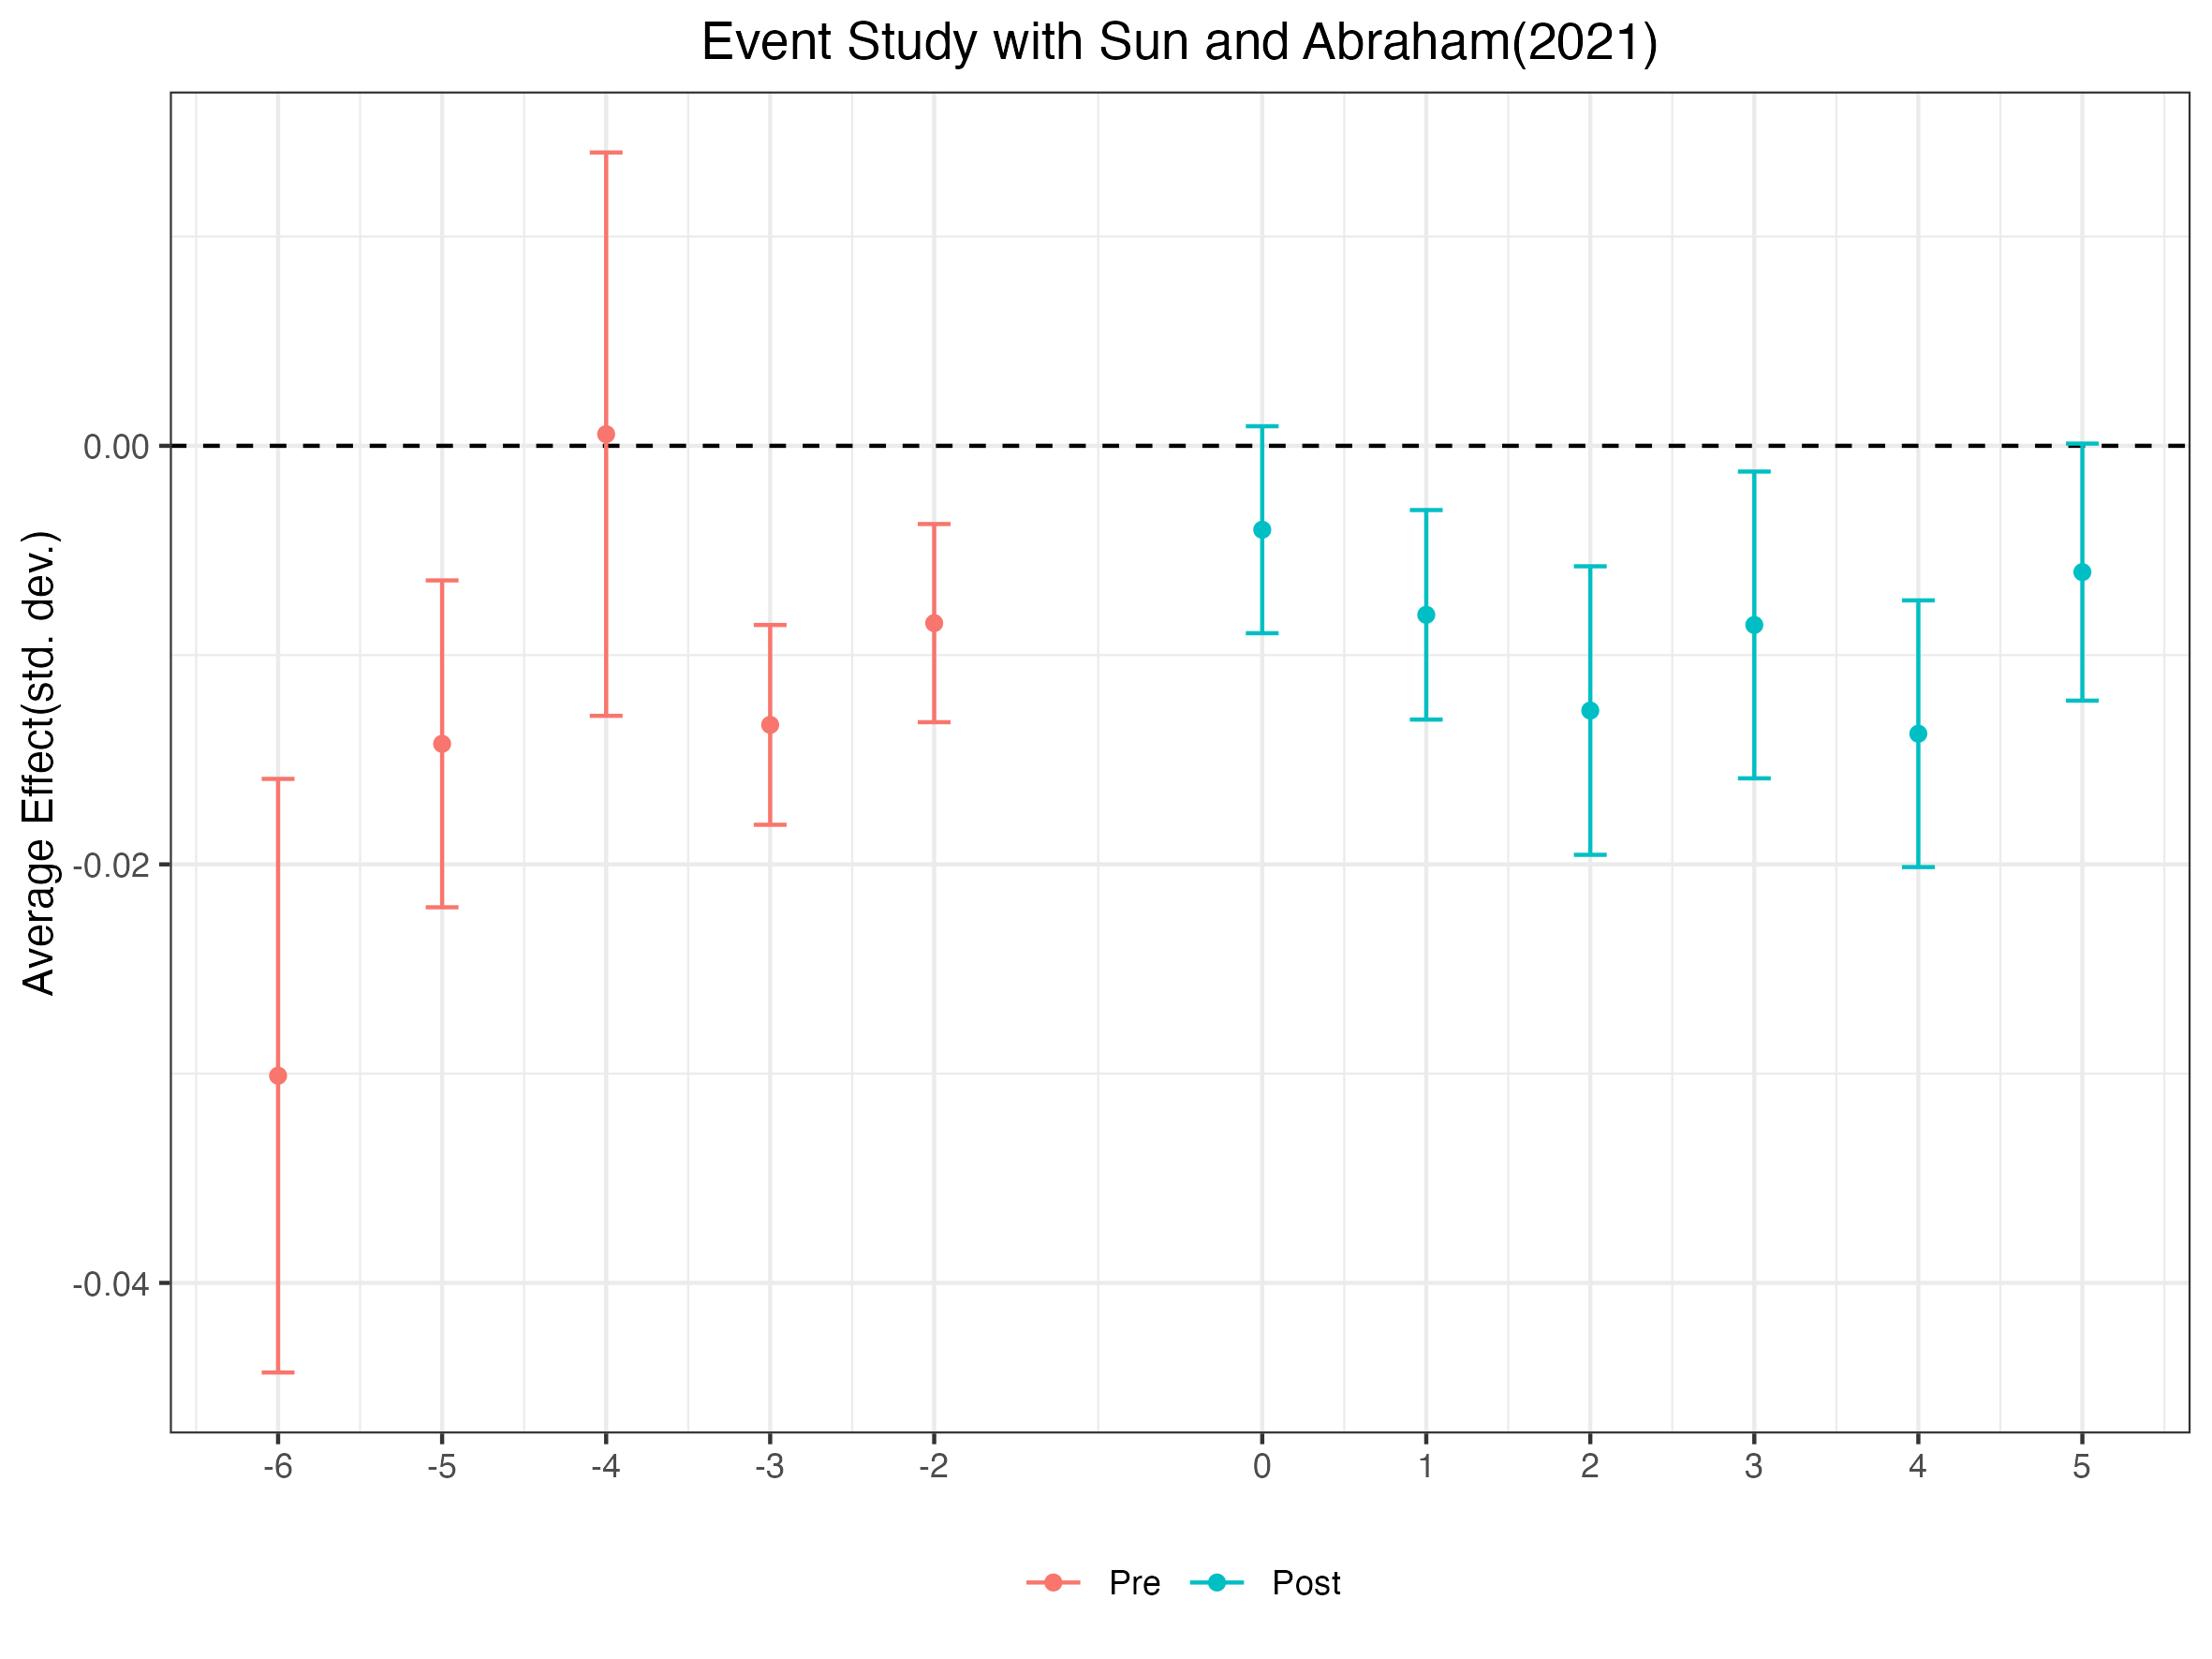
\includegraphics[width=0.7\textwidth, height=8.5cm]{figures/did-base/sadid(high school attendance).png}
    \captionsetup{width=0.7\textwidth}
    \caption{Event Study: High School Attendance}
    \label{fig:high school shares}
    \begin{minipage}{0.7\textwidth}
    \scriptsize
    Notes: The figure shows the event study results of the high school attendance among individuals between age 16 and 18 (inclusive) based on SA-DiD. 
    The base period is set to the year before the shale boom started in each state.
    The point estimates can be interpreted as the percentage point change in college enrollment status with respect to the treatment (i.e., the shale boom).
    Standard errors are clustered at the state level and the confidence intervals shown are 95\% confidence intervals.
    \end{minipage}
\end{figure}

\begin{figure}[htbp]
    \centering
    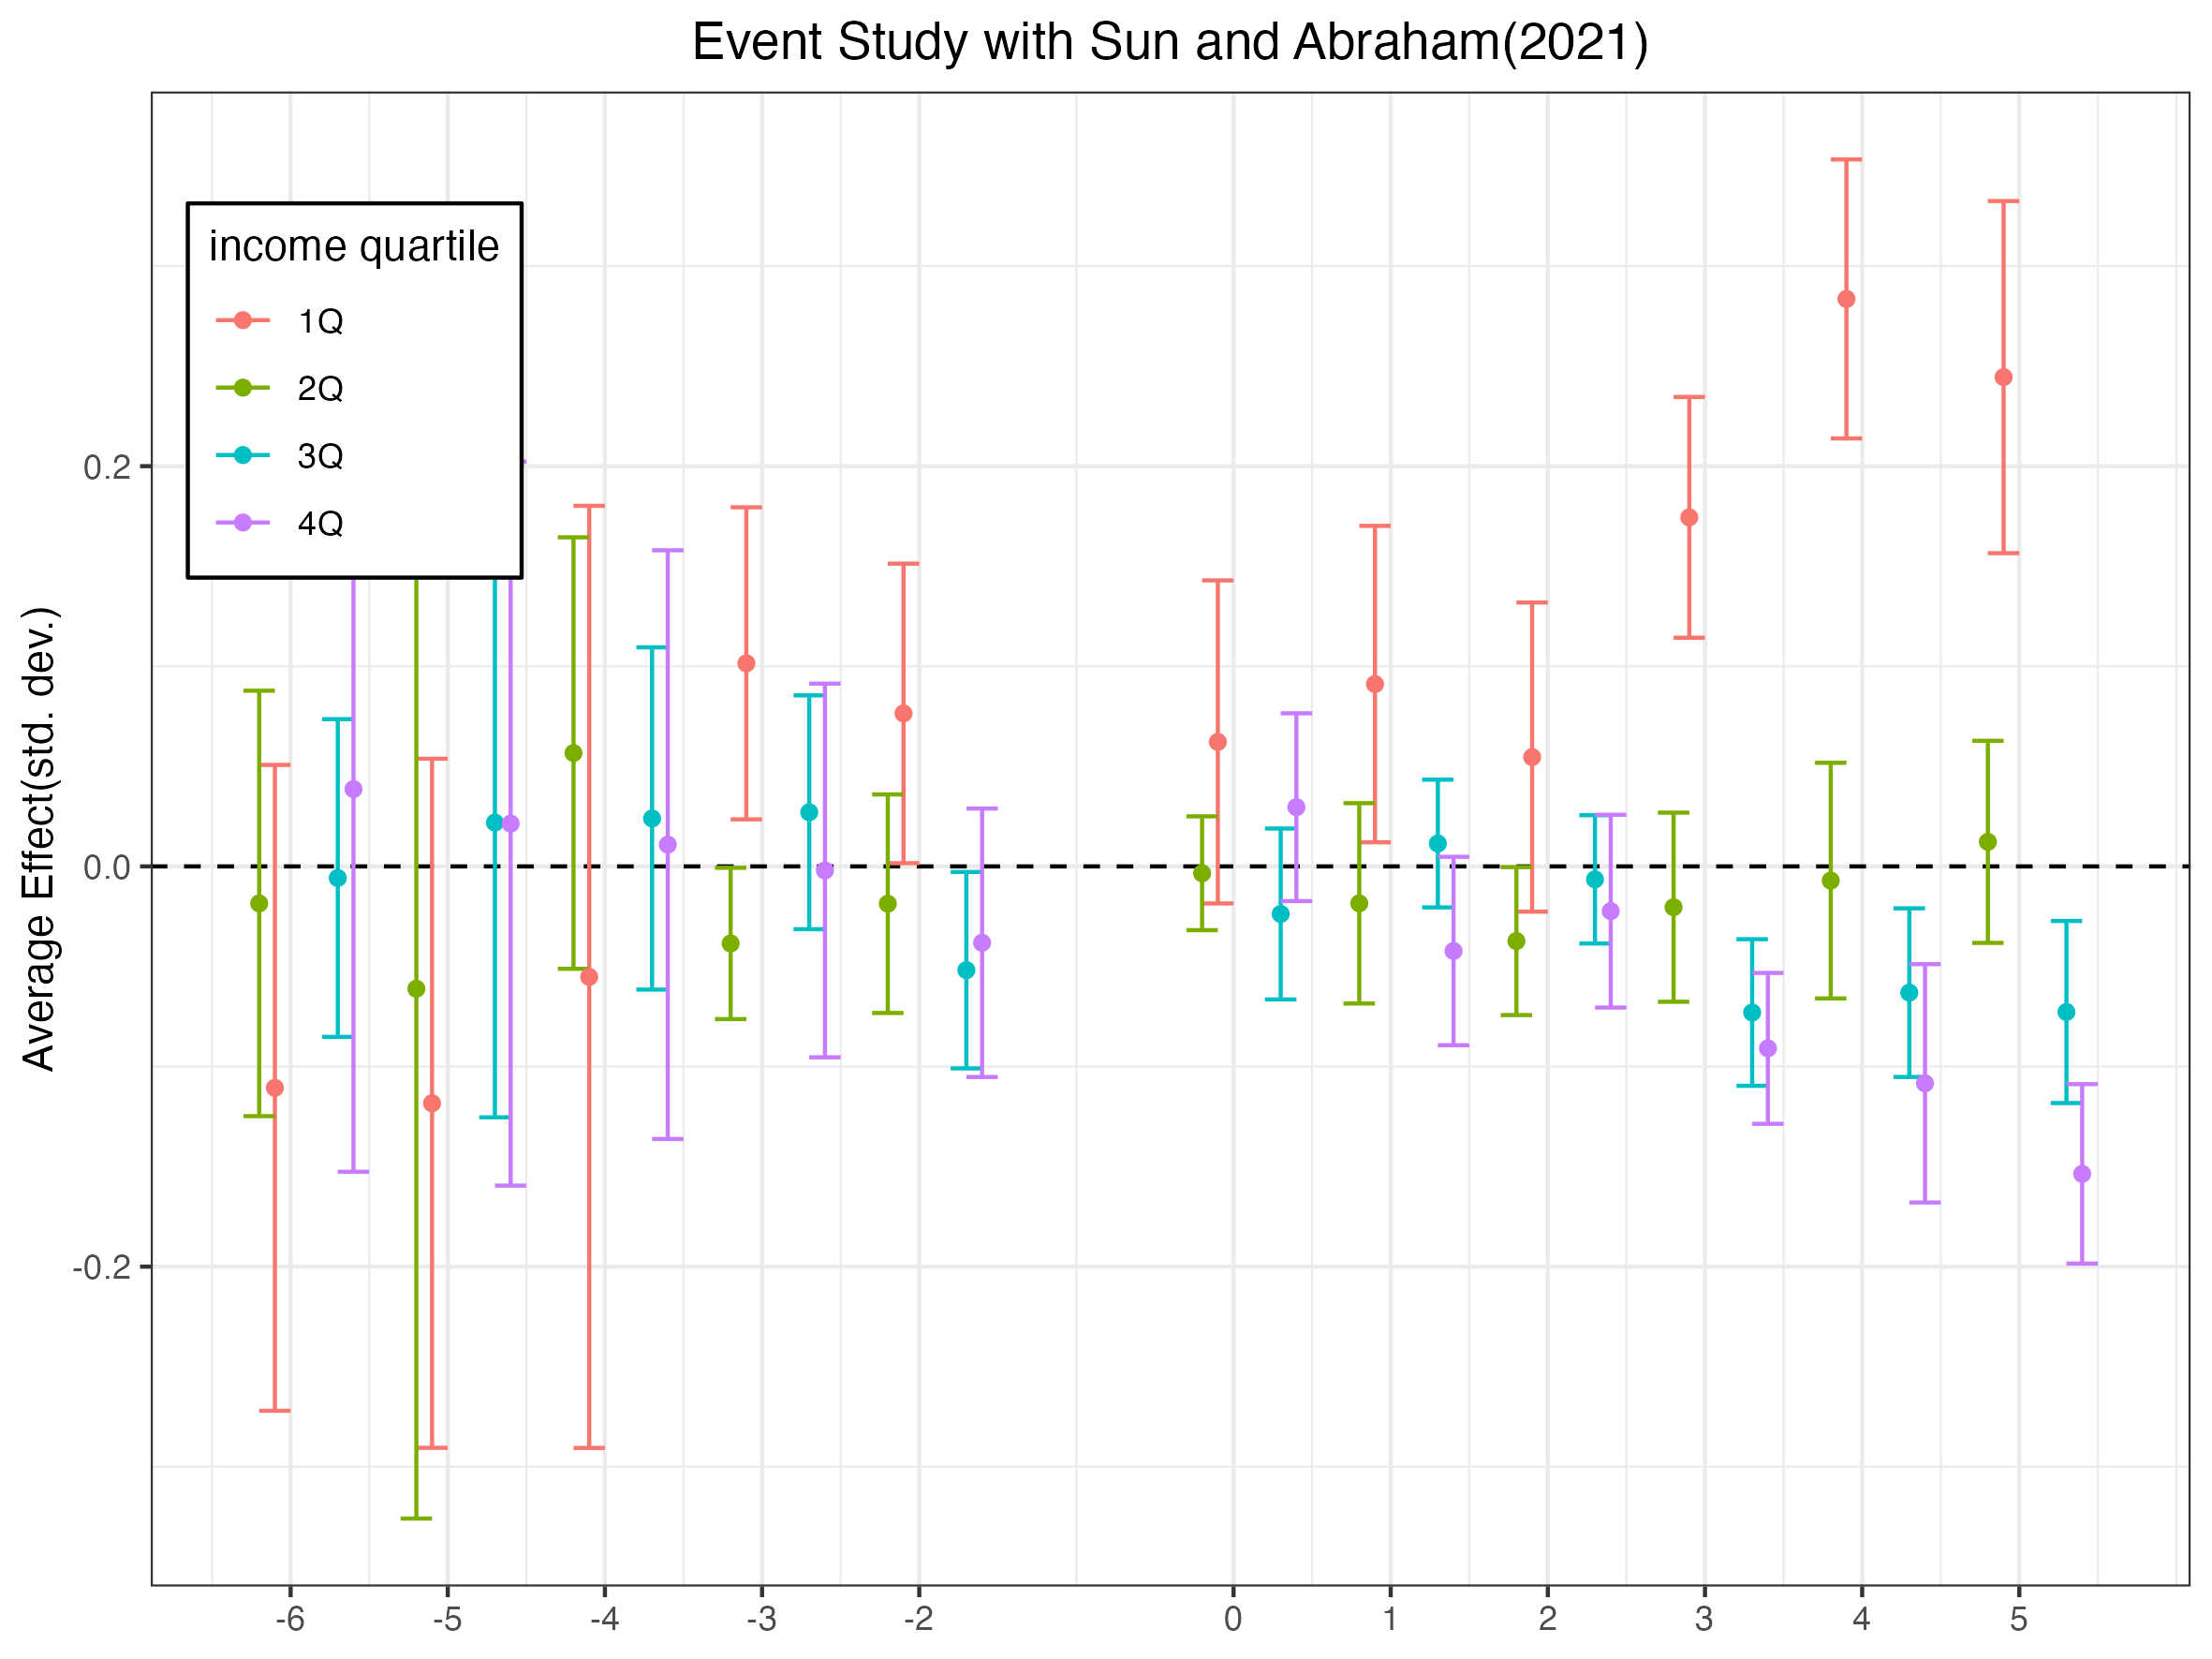
\includegraphics[width=0.7\textwidth]{figures/did-base/sadid(high school attendance- by income quartile).png}
     \captionsetup{width=0.7\textwidth}
    \caption{Event Study: High School Attendance by Household Income Quartile}
    \label{fig:high school shares - by quartile}
    \begin{minipage}{0.7\textwidth}
    \scriptsize
    Notes: The figure shows the event study results of the high school attendance among individuals between age 16 and 18 (inclusive) by family income quartile based on SA-DiD. 
    The base period is set to the year before the shale boom started in each state.
    The point estimates can be interpreted as the percentage point change in college enrollment status with respect to the treatment (i.e., the shale boom).
    Standard errors are clustered at the state level and the confidence intervals shown are 95\% confidence intervals.
    Also, note that the cutoffs for income quartiles are nation-level quartiles adjusted by the sampling weights and is fluctuant across years.
    \end{minipage}
\end{figure}


\begin{figure}[htbp]
    \centering
    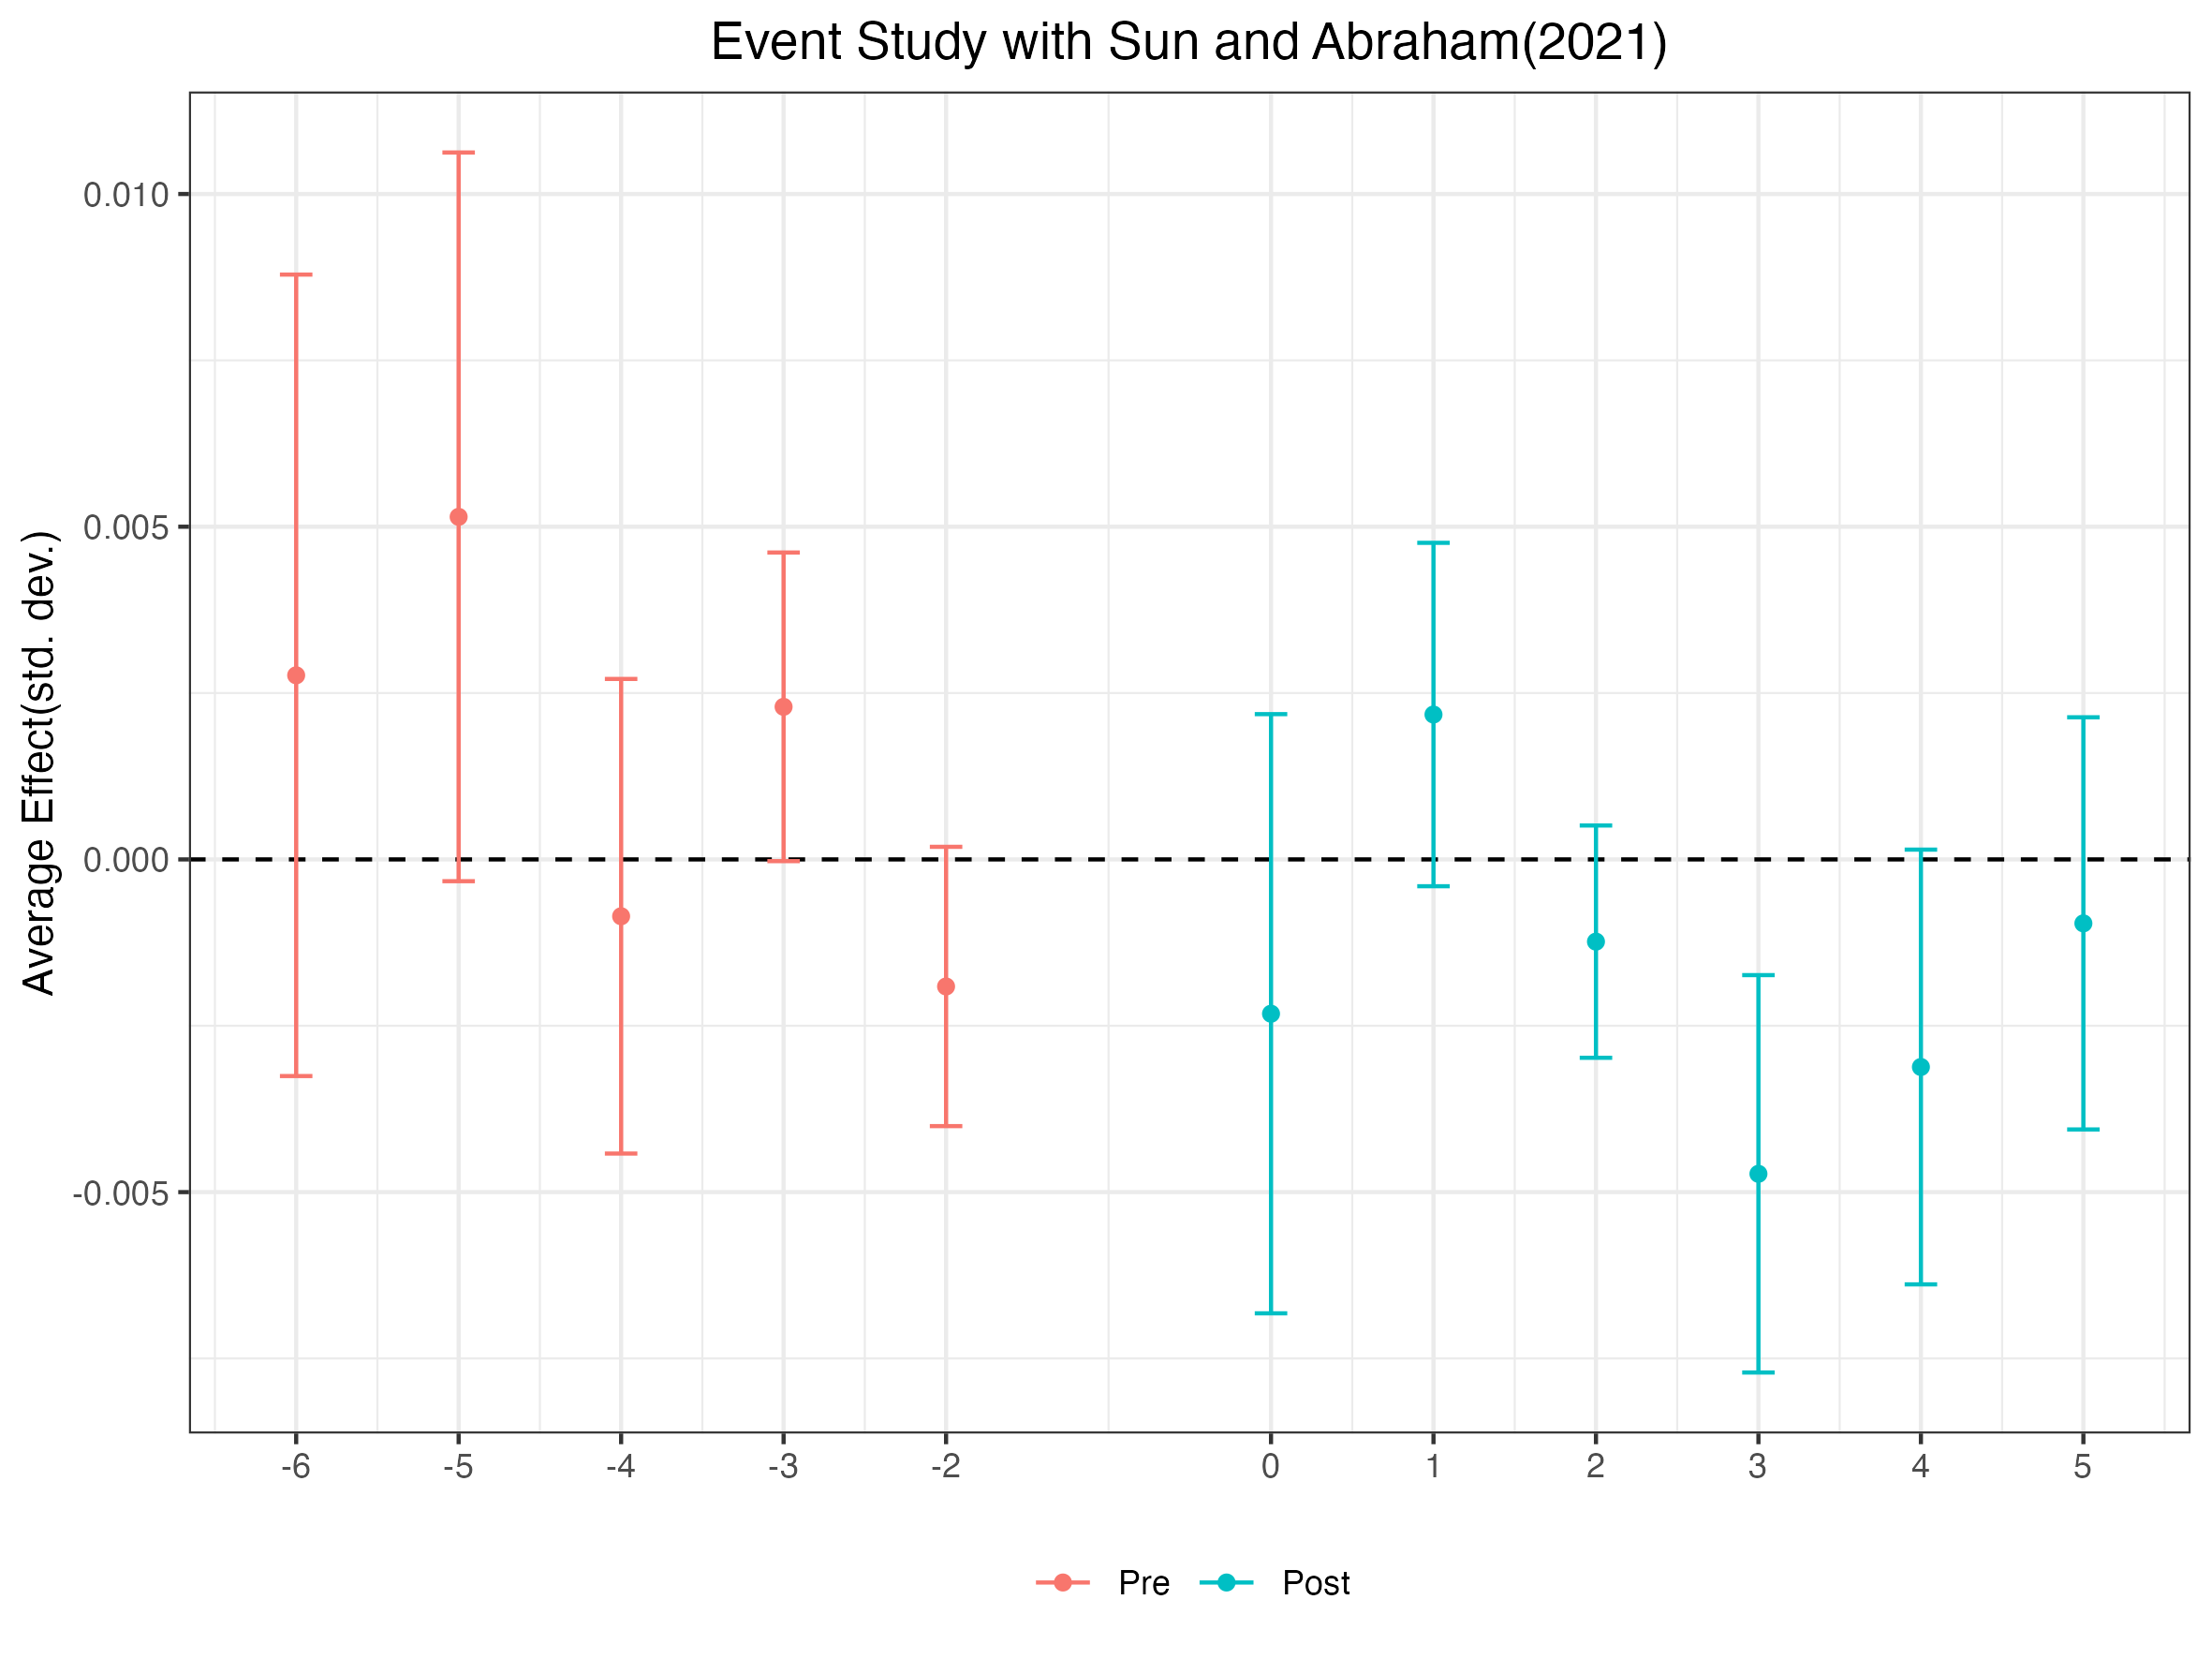
\includegraphics[width=0.7\textwidth, height=8.5cm]{figures/did-base/sadid(young school attendance).png}
     \captionsetup{width=0.7\textwidth}
    \caption{Event Study: Elementary School Attendance}
    \label{fig:elementary school shares}
    \begin{minipage}{0.7\textwidth}
    \scriptsize
     Notes: The figure shows the event study results of the elementary school attendance among individuals between age 5 and 10 (inclusive) based on SA-DiD. 
    The base period is set to the year before the shale boom started in each state.
    The point estimates can be interpreted as the percentage point change in college enrollment status with respect to the treatment (i.e., the shale boom).
    Standard errors are clustered at the state level and the confidence intervals shown are 95\% confidence intervals.
    \end{minipage}
\end{figure}

\begin{figure}[htbp]
    \centering
    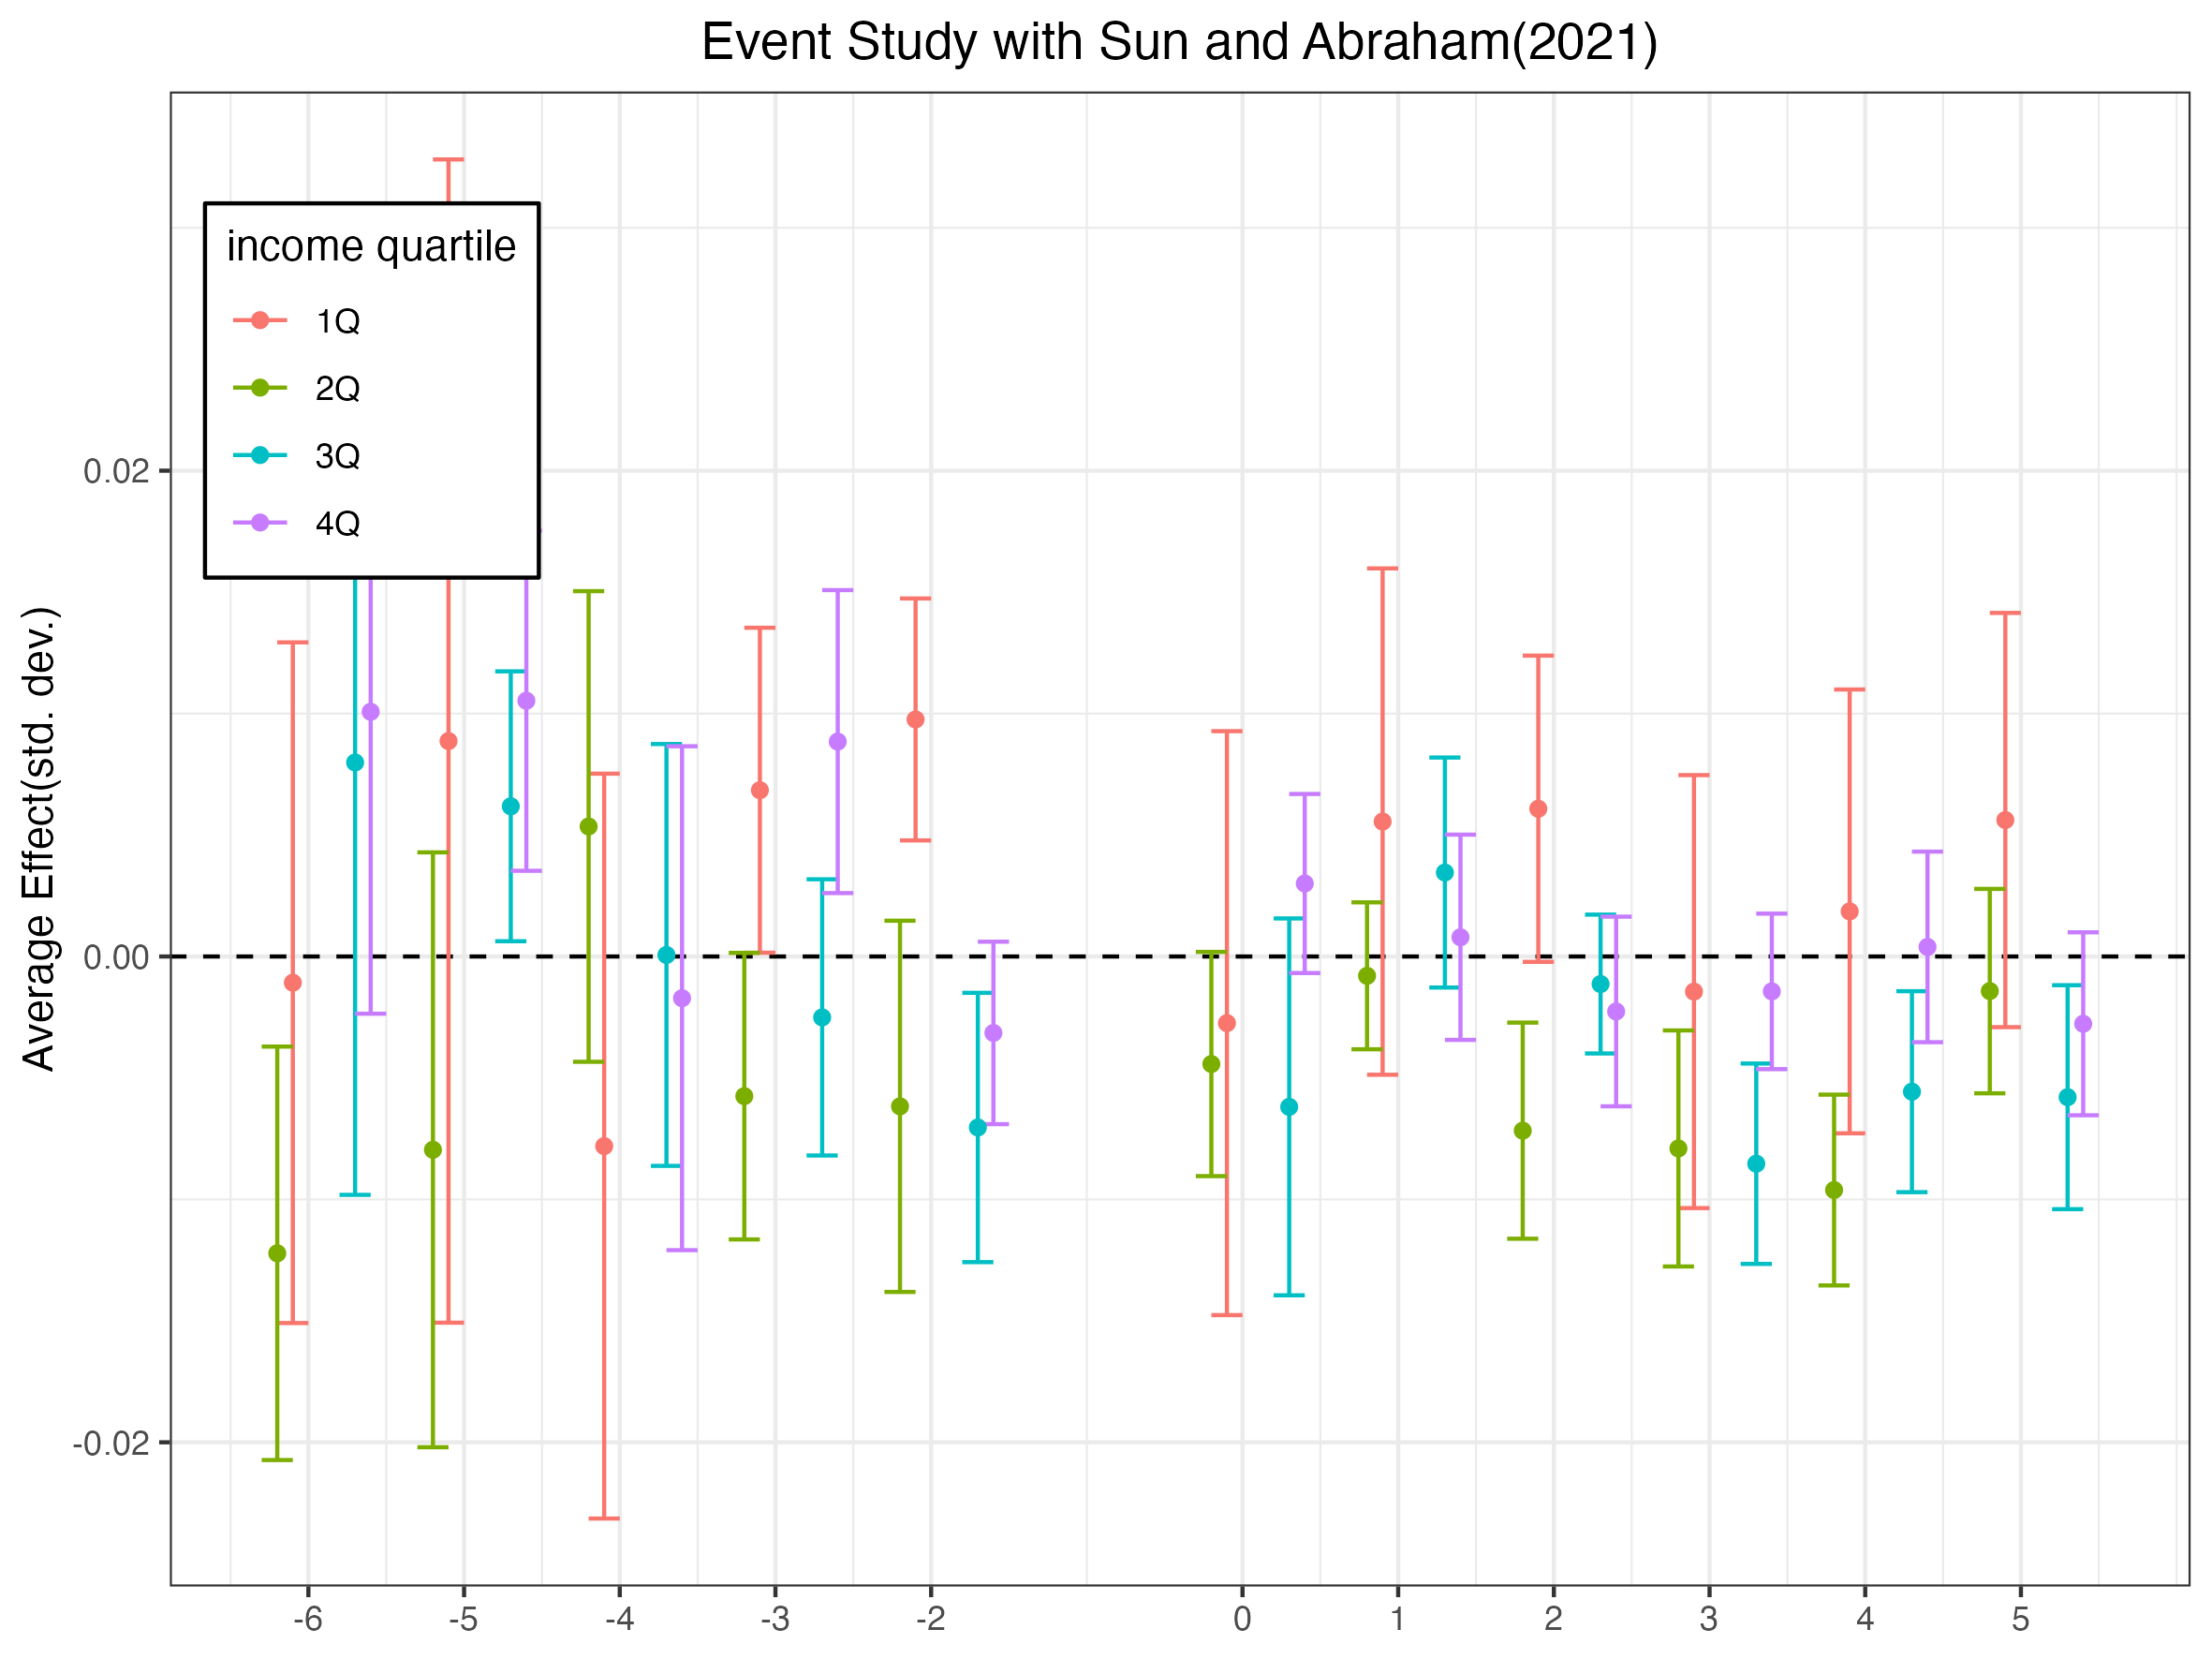
\includegraphics[width=0.7\textwidth]{figures/did-base/sadid(young school attendance - by income quartile).png}
     \captionsetup{width=0.7\textwidth}
    \caption{Event Study: Elementary School Attendance by Household Income Quartile}
    \label{fig:elementary school shares - by quartile}
    \begin{minipage}{0.7\textwidth}
    \scriptsize
    Notes: The figure shows the event study results of the elementary school attendance among individuals between age 5 and 10 (inclusive) by family income quartile based on SA-DiD. 
    The base period is set to the year before the shale boom started in each state.
    The point estimates can be interpreted as the percentage point change in college enrollment status with respect to the treatment (i.e., the shale boom).
    Standard errors are clustered at the state level and the confidence intervals shown are 95\% confidence intervals.
    Also, note that the cutoffs for income quartiles are nation-level quartiles adjusted by the sampling weights and is fluctuant across years.
    \end{minipage}
\end{figure}


\begin{figure}[htbp]
    \centering
    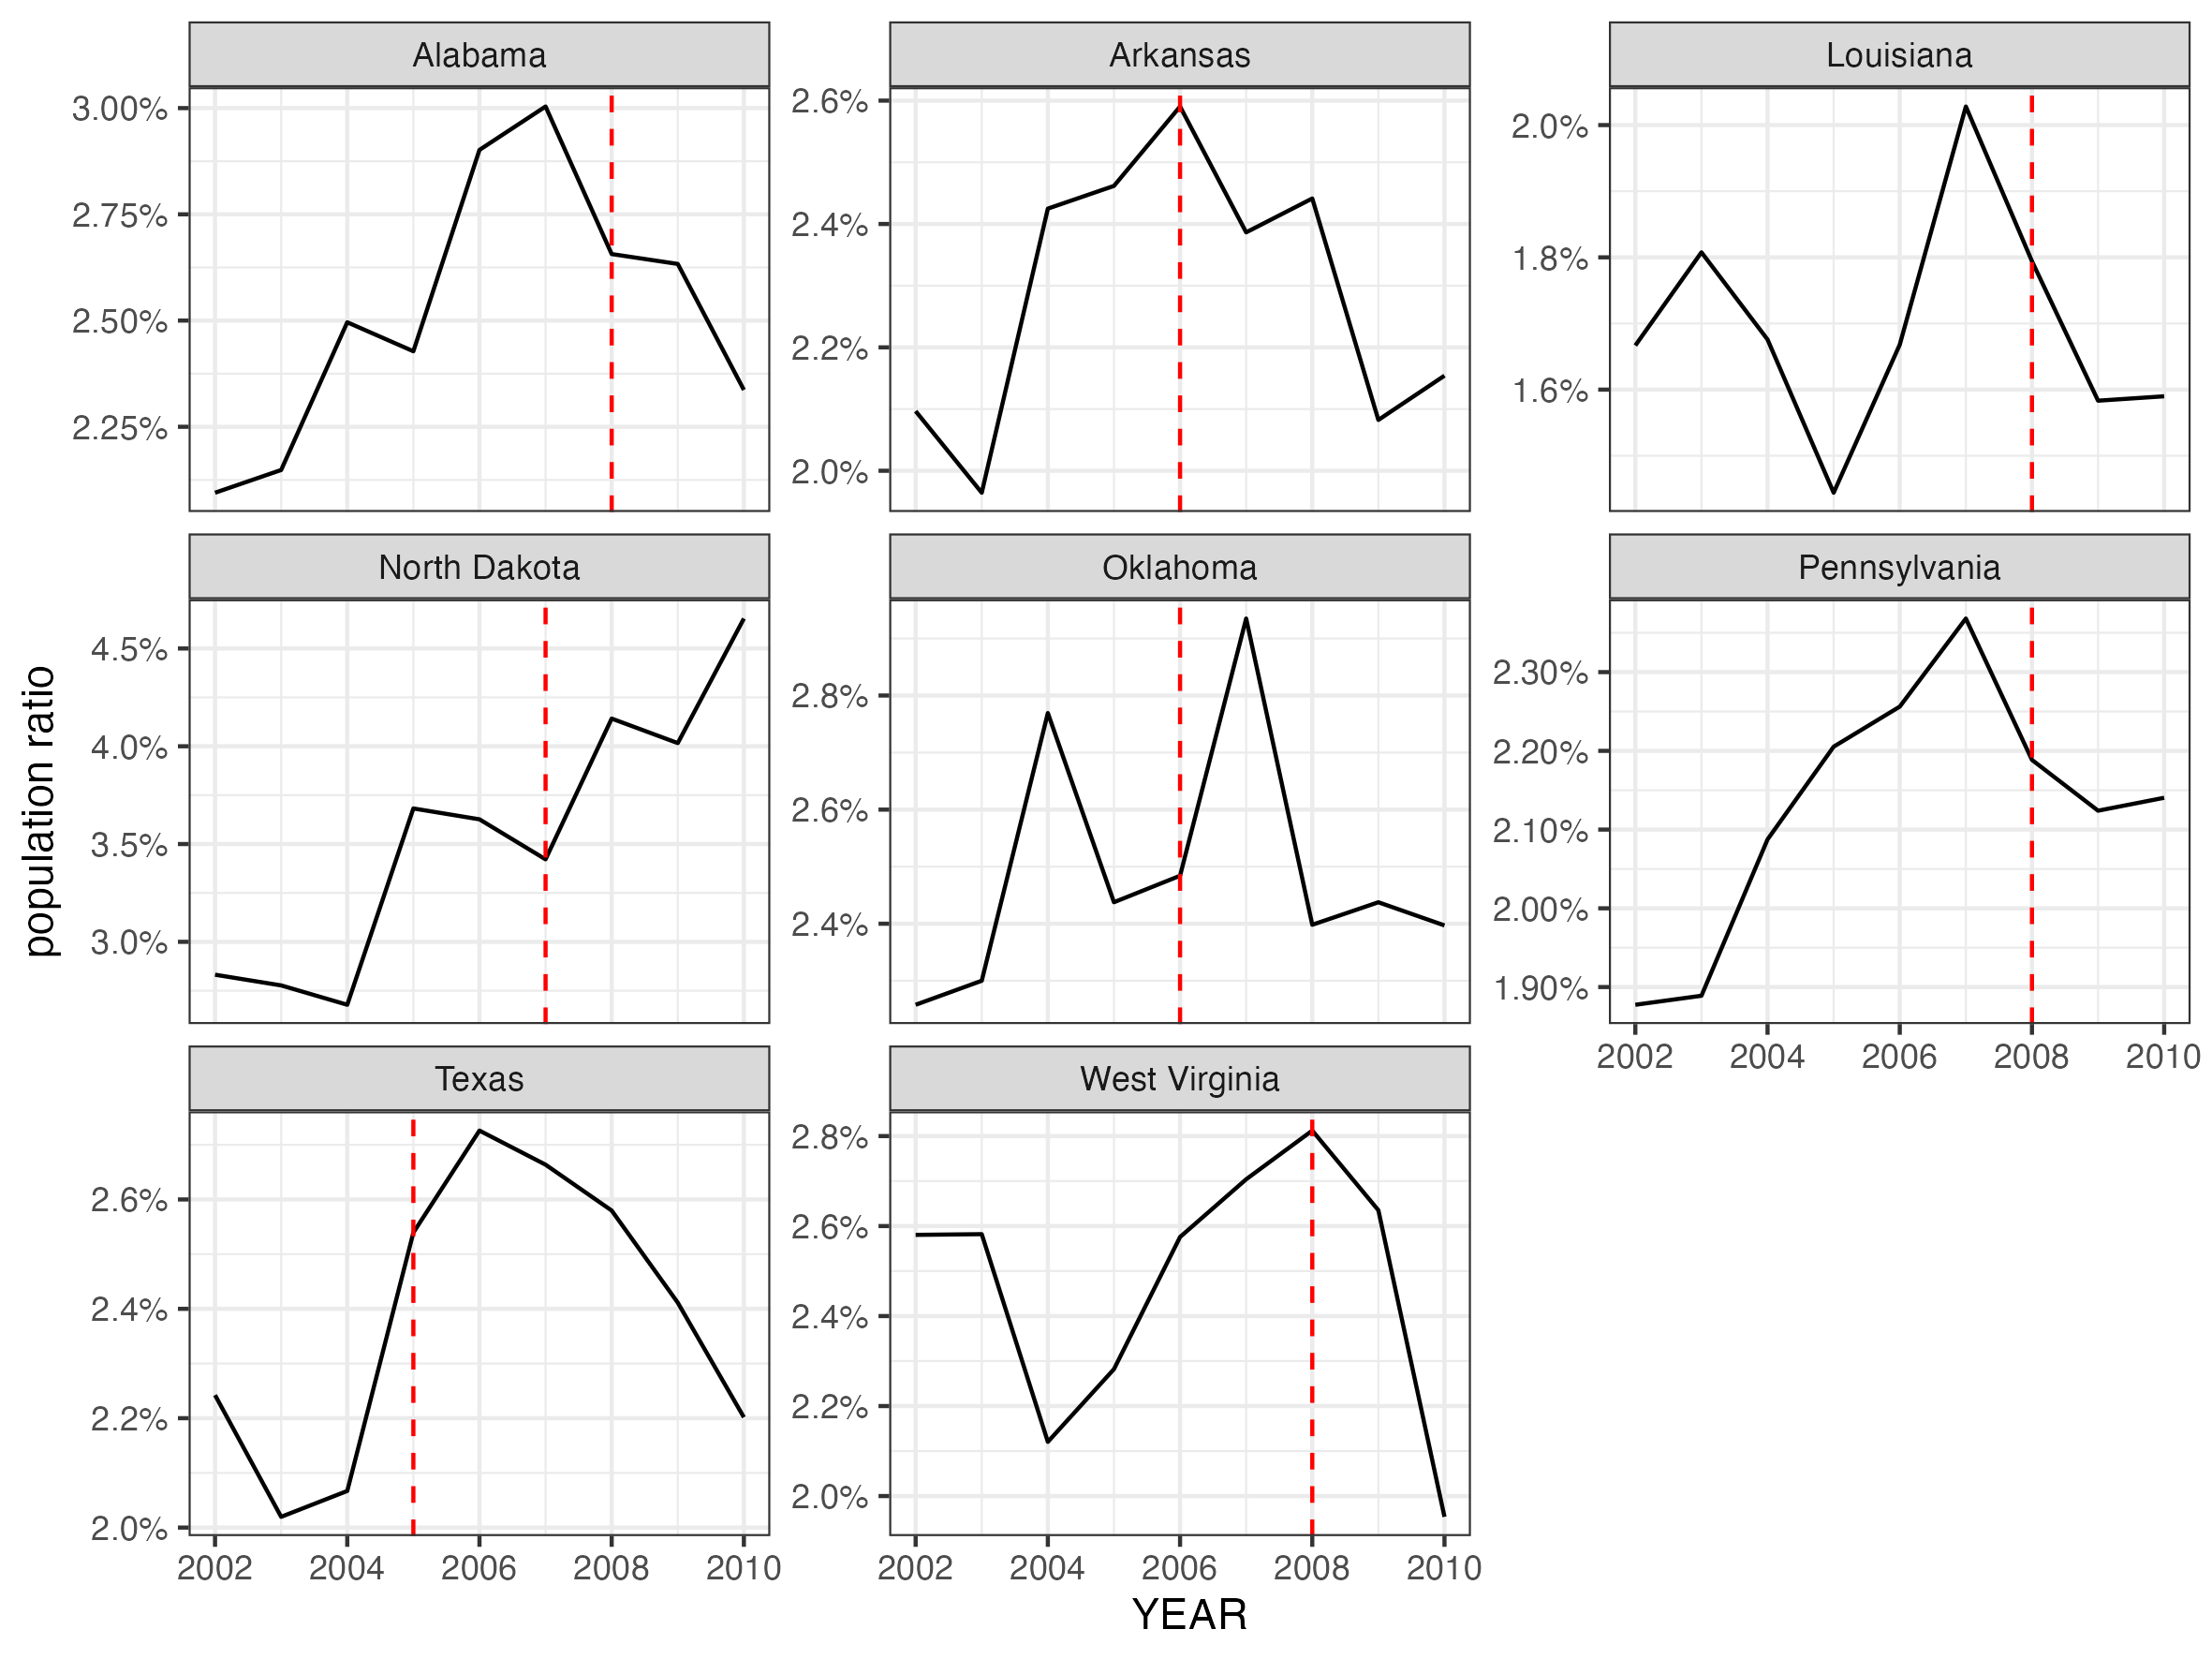
\includegraphics[width=0.7\textwidth]{figures/pop_ratio_from_outside.png}
    \captionsetup{width=0.7\textwidth}
    \caption{Population Ratio of Migrants from Outside Shale States}
    \label{fig:migration_share}
    \begin{minipage}{0.7\textwidth}
    \scriptsize
    Notes: The figure displays the population ratio of individuals who
    moved from outside the shale states to inside the shale states within a year.
    The population ratio is calculated as the (weighted) number of individuals who moved from outside the shale states to inside the shale states divided by the total population of the shale states.
    \end{minipage}
\end{figure}

\begin{figure}[htbp]
    \centering
    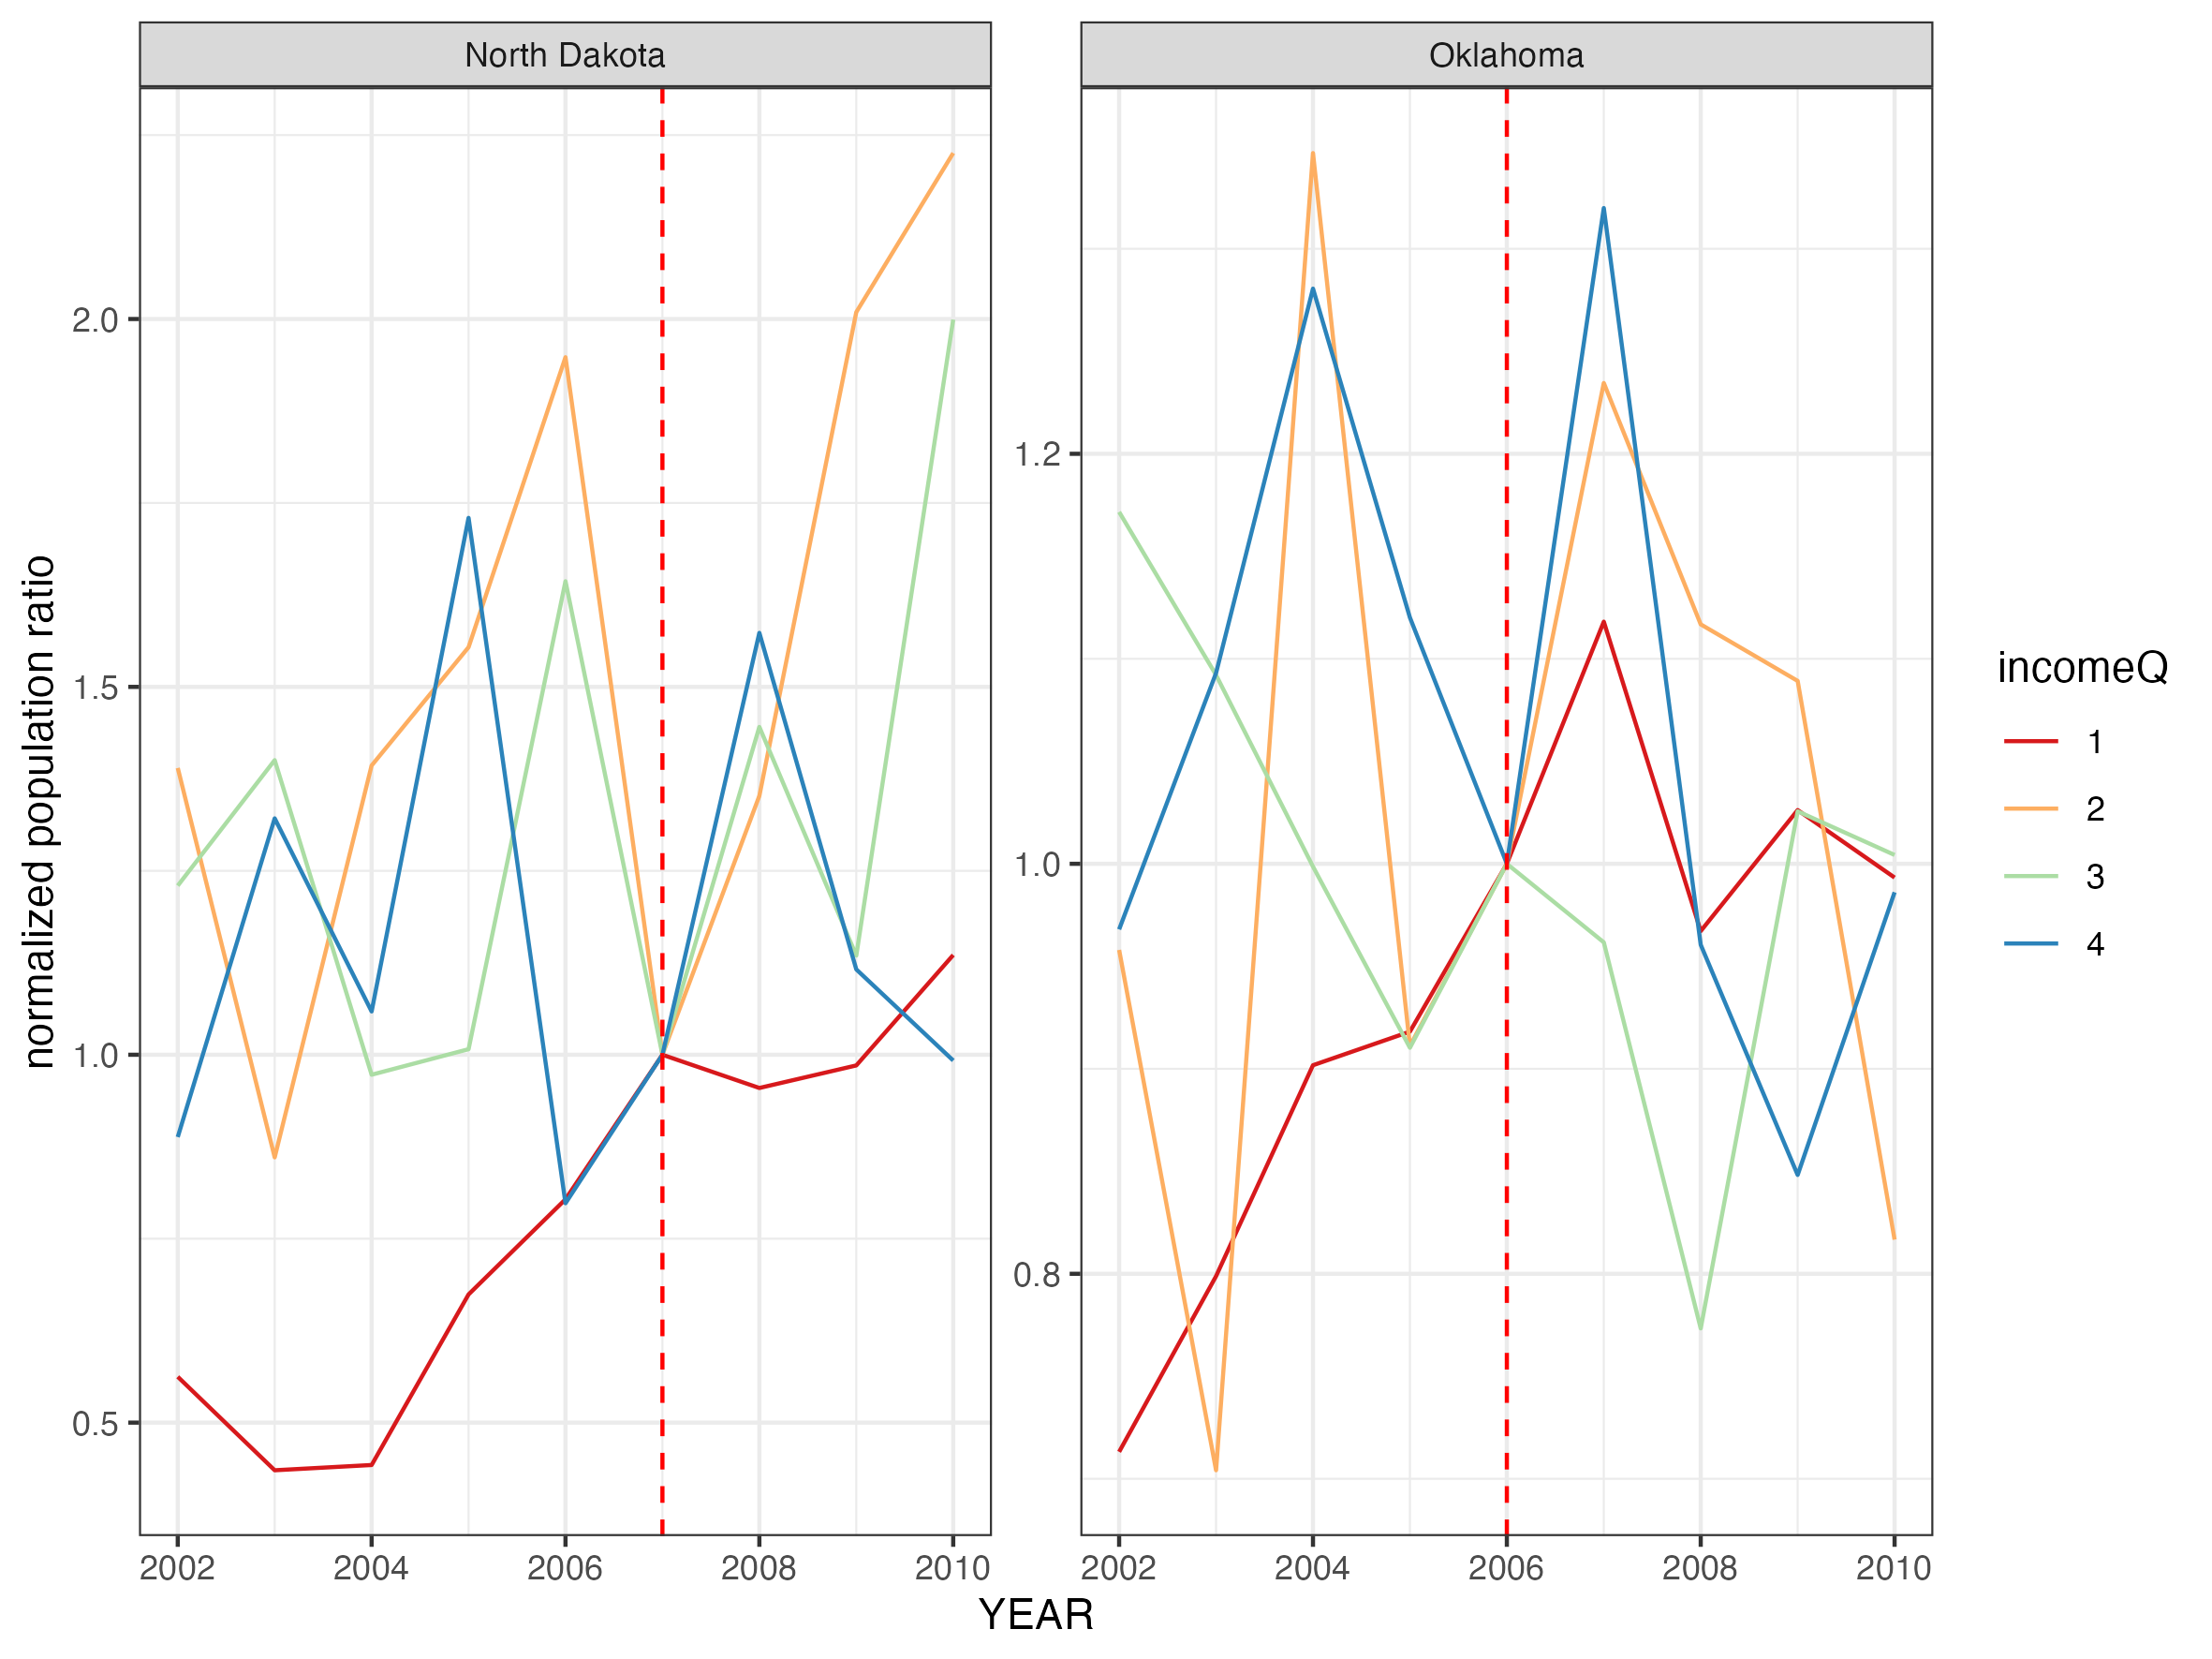
\includegraphics[width=0.7\textwidth]{figures/pop_ratio_from_outside - by income quartile.png}
    \captionsetup{width=0.7\textwidth}
    \caption{Normalized Population Ratio of Migrants from Outside Shale State by Personal Income Quartile(North Dakota and Oklahoma)}
    \label{fig:migration_share-by quartile}
    \begin{minipage}{0.7\textwidth}
    \scriptsize
    Notes: The figure displays the normalized population ratio of individuals who
    moved from outside the shale states to inside the shale states within a year.
    The normalization is done by dividing the population ratio of each income quartile group by the population ratio in the 
    year of shale boom start in each state (e.g., 2005 for Texas) – which helps focus on the relative changes in the population ratio of each income quartile group.
    Note that these income quartiles are based on personal income, not household income, and are adjusted by the sampling weights.
    The raw population ratio before normalization is calculated as the (weighted) number of individuals who moved from outside the shale states to inside the shale states divided by the total population of the shale states.
    \end{minipage}
\end{figure}


\end{document}
